% Options for packages loaded elsewhere
\PassOptionsToPackage{unicode}{hyperref}
\PassOptionsToPackage{hyphens}{url}
%
\documentclass[
]{book}
\usepackage{lmodern}
\usepackage{amssymb,amsmath}
\usepackage{ifxetex,ifluatex}
\ifnum 0\ifxetex 1\fi\ifluatex 1\fi=0 % if pdftex
  \usepackage[T1]{fontenc}
  \usepackage[utf8]{inputenc}
  \usepackage{textcomp} % provide euro and other symbols
\else % if luatex or xetex
  \usepackage{unicode-math}
  \defaultfontfeatures{Scale=MatchLowercase}
  \defaultfontfeatures[\rmfamily]{Ligatures=TeX,Scale=1}
\fi
% Use upquote if available, for straight quotes in verbatim environments
\IfFileExists{upquote.sty}{\usepackage{upquote}}{}
\IfFileExists{microtype.sty}{% use microtype if available
  \usepackage[]{microtype}
  \UseMicrotypeSet[protrusion]{basicmath} % disable protrusion for tt fonts
}{}
\makeatletter
\@ifundefined{KOMAClassName}{% if non-KOMA class
  \IfFileExists{parskip.sty}{%
    \usepackage{parskip}
  }{% else
    \setlength{\parindent}{0pt}
    \setlength{\parskip}{6pt plus 2pt minus 1pt}}
}{% if KOMA class
  \KOMAoptions{parskip=half}}
\makeatother
\usepackage{xcolor}
\IfFileExists{xurl.sty}{\usepackage{xurl}}{} % add URL line breaks if available
\IfFileExists{bookmark.sty}{\usepackage{bookmark}}{\usepackage{hyperref}}
\hypersetup{
  pdftitle={R Markdown for Psychology Graduate Students},
  pdfauthor={Holly Zaharchuk},
  hidelinks,
  pdfcreator={LaTeX via pandoc}}
\urlstyle{same} % disable monospaced font for URLs
\usepackage{color}
\usepackage{fancyvrb}
\newcommand{\VerbBar}{|}
\newcommand{\VERB}{\Verb[commandchars=\\\{\}]}
\DefineVerbatimEnvironment{Highlighting}{Verbatim}{commandchars=\\\{\}}
% Add ',fontsize=\small' for more characters per line
\usepackage{framed}
\definecolor{shadecolor}{RGB}{248,248,248}
\newenvironment{Shaded}{\begin{snugshade}}{\end{snugshade}}
\newcommand{\AlertTok}[1]{\textcolor[rgb]{0.94,0.16,0.16}{#1}}
\newcommand{\AnnotationTok}[1]{\textcolor[rgb]{0.56,0.35,0.01}{\textbf{\textit{#1}}}}
\newcommand{\AttributeTok}[1]{\textcolor[rgb]{0.77,0.63,0.00}{#1}}
\newcommand{\BaseNTok}[1]{\textcolor[rgb]{0.00,0.00,0.81}{#1}}
\newcommand{\BuiltInTok}[1]{#1}
\newcommand{\CharTok}[1]{\textcolor[rgb]{0.31,0.60,0.02}{#1}}
\newcommand{\CommentTok}[1]{\textcolor[rgb]{0.56,0.35,0.01}{\textit{#1}}}
\newcommand{\CommentVarTok}[1]{\textcolor[rgb]{0.56,0.35,0.01}{\textbf{\textit{#1}}}}
\newcommand{\ConstantTok}[1]{\textcolor[rgb]{0.00,0.00,0.00}{#1}}
\newcommand{\ControlFlowTok}[1]{\textcolor[rgb]{0.13,0.29,0.53}{\textbf{#1}}}
\newcommand{\DataTypeTok}[1]{\textcolor[rgb]{0.13,0.29,0.53}{#1}}
\newcommand{\DecValTok}[1]{\textcolor[rgb]{0.00,0.00,0.81}{#1}}
\newcommand{\DocumentationTok}[1]{\textcolor[rgb]{0.56,0.35,0.01}{\textbf{\textit{#1}}}}
\newcommand{\ErrorTok}[1]{\textcolor[rgb]{0.64,0.00,0.00}{\textbf{#1}}}
\newcommand{\ExtensionTok}[1]{#1}
\newcommand{\FloatTok}[1]{\textcolor[rgb]{0.00,0.00,0.81}{#1}}
\newcommand{\FunctionTok}[1]{\textcolor[rgb]{0.00,0.00,0.00}{#1}}
\newcommand{\ImportTok}[1]{#1}
\newcommand{\InformationTok}[1]{\textcolor[rgb]{0.56,0.35,0.01}{\textbf{\textit{#1}}}}
\newcommand{\KeywordTok}[1]{\textcolor[rgb]{0.13,0.29,0.53}{\textbf{#1}}}
\newcommand{\NormalTok}[1]{#1}
\newcommand{\OperatorTok}[1]{\textcolor[rgb]{0.81,0.36,0.00}{\textbf{#1}}}
\newcommand{\OtherTok}[1]{\textcolor[rgb]{0.56,0.35,0.01}{#1}}
\newcommand{\PreprocessorTok}[1]{\textcolor[rgb]{0.56,0.35,0.01}{\textit{#1}}}
\newcommand{\RegionMarkerTok}[1]{#1}
\newcommand{\SpecialCharTok}[1]{\textcolor[rgb]{0.00,0.00,0.00}{#1}}
\newcommand{\SpecialStringTok}[1]{\textcolor[rgb]{0.31,0.60,0.02}{#1}}
\newcommand{\StringTok}[1]{\textcolor[rgb]{0.31,0.60,0.02}{#1}}
\newcommand{\VariableTok}[1]{\textcolor[rgb]{0.00,0.00,0.00}{#1}}
\newcommand{\VerbatimStringTok}[1]{\textcolor[rgb]{0.31,0.60,0.02}{#1}}
\newcommand{\WarningTok}[1]{\textcolor[rgb]{0.56,0.35,0.01}{\textbf{\textit{#1}}}}
\usepackage{longtable,booktabs}
% Correct order of tables after \paragraph or \subparagraph
\usepackage{etoolbox}
\makeatletter
\patchcmd\longtable{\par}{\if@noskipsec\mbox{}\fi\par}{}{}
\makeatother
% Allow footnotes in longtable head/foot
\IfFileExists{footnotehyper.sty}{\usepackage{footnotehyper}}{\usepackage{footnote}}
\makesavenoteenv{longtable}
\usepackage{graphicx,grffile}
\makeatletter
\def\maxwidth{\ifdim\Gin@nat@width>\linewidth\linewidth\else\Gin@nat@width\fi}
\def\maxheight{\ifdim\Gin@nat@height>\textheight\textheight\else\Gin@nat@height\fi}
\makeatother
% Scale images if necessary, so that they will not overflow the page
% margins by default, and it is still possible to overwrite the defaults
% using explicit options in \includegraphics[width, height, ...]{}
\setkeys{Gin}{width=\maxwidth,height=\maxheight,keepaspectratio}
% Set default figure placement to htbp
\makeatletter
\def\fps@figure{htbp}
\makeatother
\usepackage[normalem]{ulem}
% Avoid problems with \sout in headers with hyperref
\pdfstringdefDisableCommands{\renewcommand{\sout}{}}
\setlength{\emergencystretch}{3em} % prevent overfull lines
\providecommand{\tightlist}{%
  \setlength{\itemsep}{0pt}\setlength{\parskip}{0pt}}
\setcounter{secnumdepth}{5}
\usepackage{booktabs}
\usepackage{amsthm}
\makeatletter
\def\thm@space@setup{%
  \thm@preskip=8pt plus 2pt minus 4pt
  \thm@postskip=\thm@preskip
}
\makeatother
\usepackage{booktabs}
\usepackage{longtable}
\usepackage{array}
\usepackage{multirow}
\usepackage{wrapfig}
\usepackage{float}
\usepackage{colortbl}
\usepackage{pdflscape}
\usepackage{tabu}
\usepackage{threeparttable}
\usepackage{threeparttablex}
\usepackage[normalem]{ulem}
\usepackage{makecell}
\usepackage{xcolor}
\usepackage[]{natbib}
\bibliographystyle{apalike}

\title{R Markdown for Psychology Graduate Students}
\author{Holly Zaharchuk}
\date{2020-05-04}

\begin{document}
\maketitle

{
\setcounter{tocdepth}{1}
\tableofcontents
}
\hypertarget{welcome}{%
\chapter{Welcome}\label{welcome}}

I designed this guide to be a resource for psychology graduate students looking to streamline their research pipelines. With R Markdown, you can load, clean, manipulate, analyze, and present your data in one environment. This guide focuses on the presentation piece, with information on creating slides, posters, manuscripts, CVs, and reports in several formats, including HTML, PDF, and Microsoft Word.

\hypertarget{background}{%
\section{Background}\label{background}}

This guide assumes a basic level of familiarity with \href{https://www.r-project.org/}{R} and \href{https://rstudio.com/products/rstudio/download/}{RStudio}. If you don't know how to use either of these, there are several \href{https://education.rstudio.com/learn/beginner/}{beginner tutorials} you should check out first. I have also created primers for Beginner and Intermediate R in Chapter \ref{supplement}.

\hypertarget{getting-started}{%
\section{Getting started}\label{getting-started}}

What is R Markdown?

\href{https://en.wikipedia.org/wiki/Markdown}{Markdown} is a specific \href{https://en.wikipedia.org/wiki/Markup_language}{markup language} with plain text-formatting syntax. \href{https://cran.r-project.org/web/packages/stationery/vignettes/Rmarkdown.pdf}{R Markdown} is a specific markdown variety.

R Markdown and R are not the same thing. R Markdown combines R code (or code from other programming languages) and markdown in the RStudio integrated development environment (IDE). This allows you to embed code and text in the same document.

You can install the \texttt{rmarkdown} package from CRAN or GitHub:

\begin{Shaded}
\begin{Highlighting}[]
\KeywordTok{install.packages}\NormalTok{(}\StringTok{"rmarkdown"}\NormalTok{)}
\CommentTok{# or the development version:}
\CommentTok{# devtools::install_github("rstudio/rmarkdown")}
\end{Highlighting}
\end{Shaded}

\hypertarget{tips}{%
\subsection{Tips}\label{tips}}

\begin{itemize}
\tightlist
\item
  Treat your data as read-only
\item
  Comment code early and often
\item
  Keep code chunks small
\item
  Label chunks to help with diagnosing issues
\item
  Nest all files under one directory (if possible)
\end{itemize}

\hypertarget{general-reference-documents}{%
\subsection{General reference documents}\label{general-reference-documents}}

\begin{itemize}
\tightlist
\item
  \href{https://bookdown.org/yihui/rmarkdown/}{R Markdown Guide}
\item
  \href{https://rstudio.com/wp-content/uploads/2016/03/rmarkdown-cheatsheet-2.0.pdf}{R Markdown Cheat Sheet}
\item
  \href{https://rstudio.com/wp-content/uploads/2015/03/rmarkdown-reference.pdf}{R Markdown Reference Guide}
\item
  \href{https://support.rstudio.com/hc/en-us/articles/200711853-Keyboard-Shortcuts}{Keyboard shortcuts}
\item
  \href{https://yihui.org/knitr/}{\texttt{knitr} documentation}
\end{itemize}

\hypertarget{intro}{%
\chapter{Parts of a document}\label{intro}}

\begin{enumerate}
\def\labelenumi{\arabic{enumi}.}
\tightlist
\item
  YAML header
\item
  Markdown
\item
  Code chunks
\end{enumerate}

\hypertarget{yaml-header}{%
\section{YAML header}\label{yaml-header}}

The first part of your document is called the YAML header. This is where you set the global options for the output and formatting. The YAML header appears at the top of your document, and is defined by three dashes/hyphens at the beginning and end.

In the example below, I show the YAML header for a set of \texttt{revealjs} slides. I've included basic information, like the title and date, in addition to template-specific parameters, like whether there should be slide numbers or not. Section \ref{yamlref} has more information on setting YAML formatting parameters.

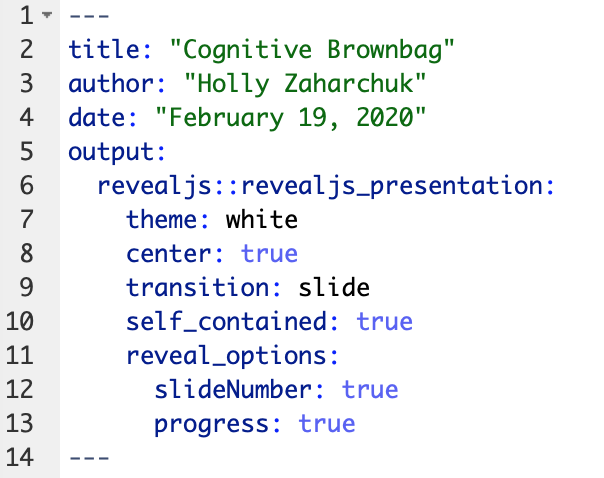
\includegraphics[width=8.39in]{images/example_yaml}

\hypertarget{markintro}{%
\section{Markdown}\label{markintro}}

The plain text-formatting syntax of R Markdown allows for conversion to multiple document types. The image below shows an example of the basic syntax. The \# denotes a header, while the numbered list behaves like you would expect one to in Word. However, unlike Word, the actual numbers don't matter; I could've put all 1's here, and R Markdown would've formatted them for me. Go to Chapter \ref{content} for more information on markdown syntax.

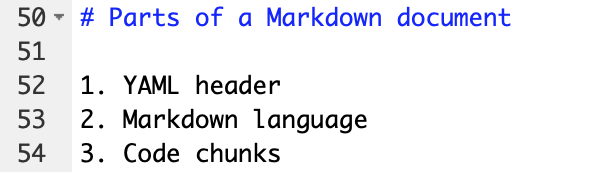
\includegraphics[width=8.22in]{images/example_markdown}

\hypertarget{chunkex}{%
\section{Code chunks}\label{chunkex}}

Code chunks are one of the core features of R Markdown. Code chunks are set apart from markdown by three backticks at the beginning and end. In curly brackets after the first set of backticks, you specify the coding language you want to use (here, it's R, with a lowercase r).

You can also add other arguments, like a name for the chunk (here, it's \texttt{setup}), and specific chunk options. The example I've provided below is the first chunk in my R Markdown document. It establishes the default chunk options with \texttt{knitr::opts\_chunk\$set}. You can see that while I've set \texttt{echo\ =\ TRUE} globally, so that all of my code chunks appear in the document by default, I set \texttt{echo\ =\ FALSE} for this specific chunk. A full list of chunk options can be found \href{https://rstudio.com/wp-content/uploads/2015/03/rmarkdown-reference.pdf}{here}.

\begin{Shaded}
\begin{Highlighting}[]
\CommentTok{# This is a chunk of R code that adds an image}
\NormalTok{knitr}\OperatorTok{::}\KeywordTok{include_graphics}\NormalTok{(}\StringTok{"images/example_chunk.png"}\NormalTok{)}
\end{Highlighting}
\end{Shaded}

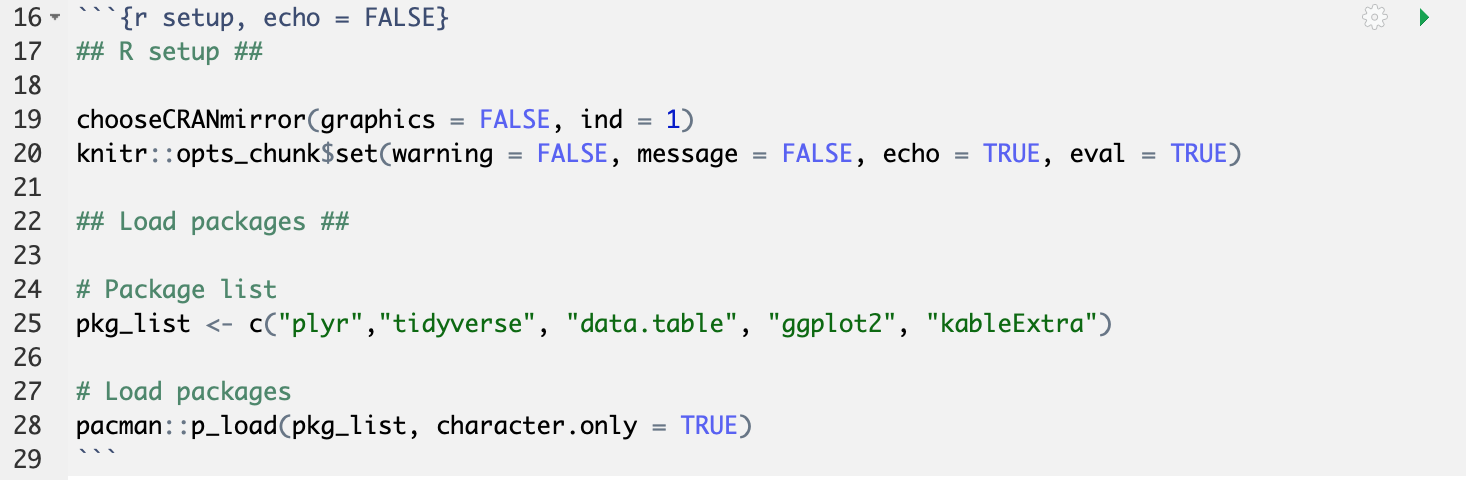
\includegraphics[width=20.36in]{images/example_chunk}

There are multiple ways to run code chunks to test them in RStudio before creating your output. You can run code like you would in R by highlighting the relevant lines of code and hitting CTRL/command + enter. You can also hit the green ``play'' button in the upper right-hand corner of the chunk.

Each chunk is an island, so if you haven't run a previous chunk that contains some variable you need in the chunk you want to run, it'll throw an error. At the top right of your open .Rmd document in RStudio, you'll also see a \textbf{Run} dropdown menu. There, you can choose different options for running certain code chunks.

Tip: you can use the chunk option ``cache = TRUE'' for very time-consuming chunks, but there are some catches as described \href{https://bookdown.org/yihui/rmarkdown-cookbook/cache.html}{here}.

\hypertarget{output}{%
\chapter{Outputs}\label{output}}

R Markdown can transform plain text and code into several different document formats. There are also multiple ways to \textbf{Knit} or \texttt{render} the output.

\hypertarget{output-options}{%
\section{Output options}\label{output-options}}

\hypertarget{html_document}{%
\subsection{html\_document}\label{html_document}}

HTML is overall the most flexible. It supports the types of content we're interested in creating as graduate students---tables, graphs, and the like---and you can easily transform your HTML output to a PDF with \texttt{pagedown::chrome\_print(file)} if you have Google Chrome. The \href{https://github.com/brentthorne/posterdown}{poster template} I use follows this process.

\hypertarget{pdf_document}{%
\subsection{pdf\_document}\label{pdf_document}}

If you're familiar with LaTeX, you may be inclined to output directly to a PDF, since you can include inline LaTeX code in your documents (more on this in Chapter \ref{format}). The \href{https://github.com/mitchelloharawild/vitae}{CV} and \href{https://github.com/rosannav/thesis_in_rmarkdown/tree/master/example_thesis}{manuscript} templates that I use rely on the fine-grained typsetting capabilities of LaTeX. To create a PDF, you need to have LaTeX installed locally. If you don't already, you can install a \href{https://yihui.org/tinytex/}{\texttt{tinytex}} distribution through the R console.

\begin{Shaded}
\begin{Highlighting}[]
\KeywordTok{install.packages}\NormalTok{(}\StringTok{"tinytex"}\NormalTok{)}
\end{Highlighting}
\end{Shaded}

\hypertarget{word_document}{%
\subsection{word\_document}\label{word_document}}

You can also output to Microsoft Word and Powerpoint. I often work with colleagues who prefer to edit in Word, so sometimes I need to do this. I prefer not to if I can help it though, because you lose several important functions. For example, chunk options for aligning and setting the size of graphs and other images don't work, and \texttt{kable} tables tend not to appear correctly.

\hypertarget{rendering-options}{%
\section{Rendering options}\label{rendering-options}}

\hypertarget{knit}{%
\subsection{Knit}\label{knit}}

You can specify a particular output type in the YAML header with the \textbf{output} option. Then, you can press the \textbf{Knit} button or CTRL/command + shift + K to create or ``knit'' the document.

Be sure to pay attention to indentation and colon placement in your YAML header, especially as you start to specify options for particular output types. As a rule of thumb, if you have anything more than \textbf{output: output\_format}, you need to indent every new line, and have a colon at the end of the previous line. See Section \ref{usedef} for an example of this.

\hypertarget{rmarkdownrender}{%
\subsection{\texorpdfstring{\texttt{rmarkdown::render}}{rmarkdown::render}}\label{rmarkdownrender}}

Instead of knitting, you can also render files in the console with \texttt{rmarkdown::render(file,\ output\_format)}. This is essentially what \textbf{Knit} is doing. This approach allows you to create multiple output types quickly and easily. I'm usually customizing my output very specifically for one output type by adding inline CSS or LaTeX code, so I really only use \texttt{render} when I'm making \href{https://rmarkdown.rstudio.com/developer_parameterized_reports.html\%23parameter_types\%2F}{parameterized reports}.

\hypertarget{rendering-process}{%
\section{Rendering process}\label{rendering-process}}

When you \textbf{Knit} or \texttt{render} your document, there's a particular sequence of events that happens under the hood. Your R Markdown document is piped through to pandoc by the \texttt{knitr} package, which runs your code chunks and knits them together with the plain text you've included. Pandoc ultimately handles the conversion to a particular output format. Understanding this process can help you troubleshoot when you run into issues. You can find more on troubleshooting in Chapter \ref{trouble}.

\begin{figure}
\centering
\includegraphics{https://rosannavanhespenresearch.files.wordpress.com/2016/03/pandoc1.png}
\caption{Knitting process from \href{https://www.rosannavanhespen.nl/thesis_in_rmarkdown/}{Writing Your Thesis with R Markdown}}
\end{figure}

\hypertarget{template}{%
\chapter{Templates}\label{template}}

\begin{enumerate}
\def\labelenumi{\arabic{enumi}.}
\tightlist
\item
  Built-in templates
\item
  Templates from R packages
\item
  User-defined templates
\end{enumerate}

\hypertarget{built-in-templates}{%
\section{Built-in templates}\label{built-in-templates}}

R Markdown has several output templates built in, and you just have to specify them with the YAML \textbf{output} parameter. These include:

\begin{itemize}
\tightlist
\item
  \href{https://rmarkdown.rstudio.com/lesson-11.html}{Presentations}

  \begin{itemize}
  \tightlist
  \item
    ioslides and Slidy for HTML
  \item
    Beamer for PDF
  \end{itemize}
\item
  Interactive \href{https://bookdown.org/yihui/rmarkdown/shiny-documents.html}{Shiny} documents and presentations
\end{itemize}

\hypertarget{packages}{%
\section{Templates from R packages}\label{packages}}

You can also download specific templates from CRAN and GitHub. You use them the same way as the built-in templates by specifying them in the YAML header. A few that I've used or played with include:

\begin{itemize}
\tightlist
\item
  Presentations: \href{https://cran.r-project.org/web/packages/revealjs/index.html}{\texttt{revealjs}}
\item
  CVs: \href{https://github.com/mitchelloharawild/vitae}{\texttt{vitae}}
\item
  Academic posters: \href{https://github.com/brentthorne/posterdown}{\texttt{posterdown}}
\item
  APA articles: \href{https://github.com/crsh/papaja}{\texttt{papaja}}
\item
  Journal templates: \href{https://bookdown.org/yihui/rmarkdown/rticles-templates.html}{\texttt{rticles}}
\item
  HTML theme: \href{https://github.com/yixuan/prettydoc}{\texttt{prettydoc}}
\end{itemize}

\hypertarget{usedef}{%
\section{User-defined templates}\label{usedef}}

There are also ways to include templates for other output types in the YAML header.

\hypertarget{pdf}{%
\subsection{PDF}\label{pdf}}

For PDFs, you can include LaTeX templates, but you need to pay attention to the use of \$. The PLOS template shown in the image below failed to compile when I first downloaded it, because \$ are special characters for pandoc. After I added a second \$ throughout the document (you just use find and replace for this), it worked. See Section \ref{latexpacks} for calling specific LaTeX packages in R Markdown.

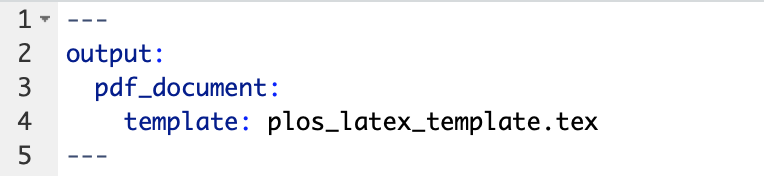
\includegraphics[width=10.61in]{images/template_latex}

\hypertarget{word}{%
\subsection{Word}\label{word}}

You can also set up Word templates. To do this, you need to use the Styles Pane in the Word Document you want to use as a template. Highlight the text you want to format, make the desired changes, then find the style that applies to that section, and find ``Update to Match Selection'' in the dropdown menu.

In the example below, you can see that I'm editing the ``Title'' format, so I need to update that particular entry in the Styles Pane. You have to do this for every text element in the document, but once you've set it up once this way, you can simply include it the same way as the LaTeX template shown above.

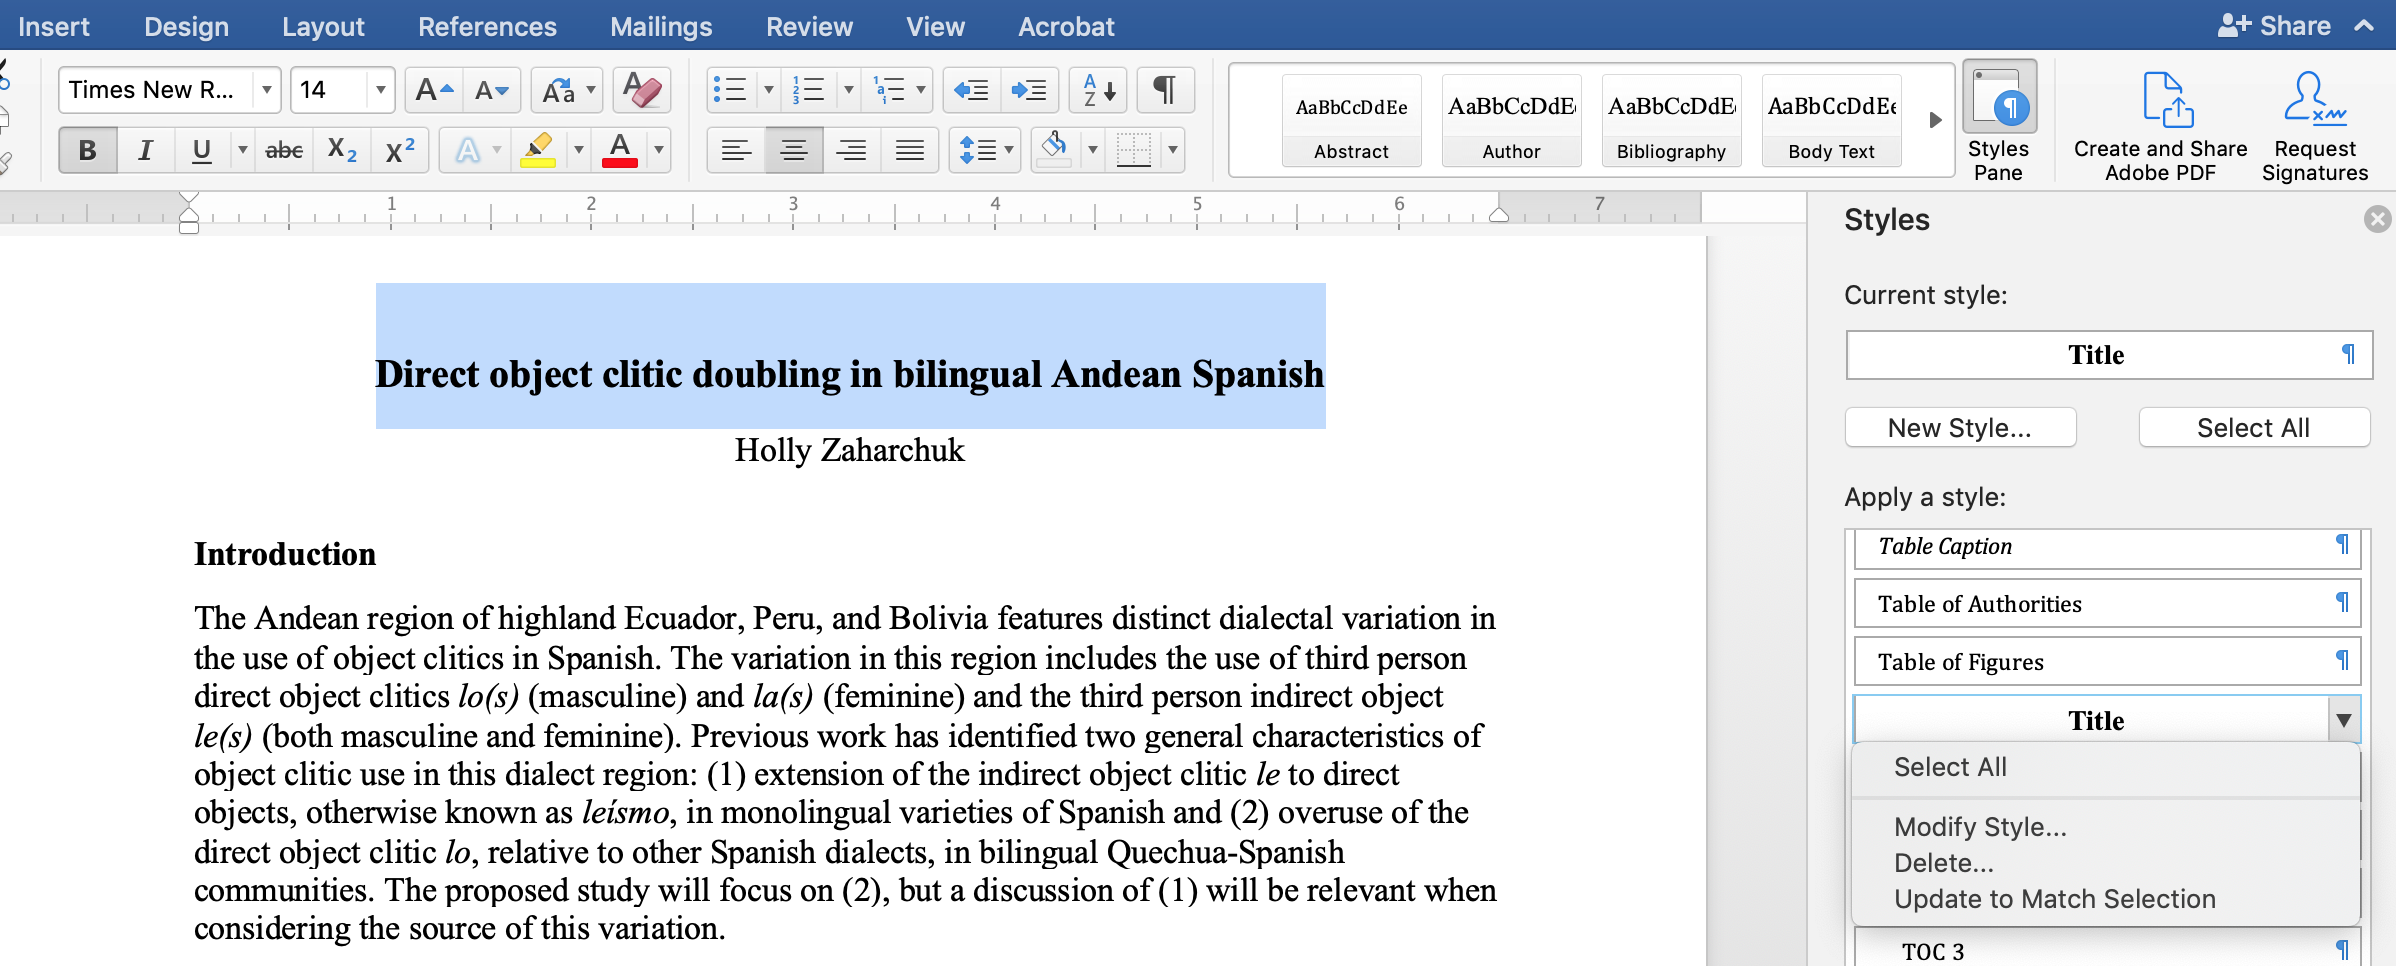
\includegraphics[width=33.28in]{images/template_word}

\hypertarget{content}{%
\chapter{Content}\label{content}}

The content of an R Markdown document includes the markdown text itself, as well as output from code chunks. Code chunks can output data, graphs, tables, and images. You can also reference variables from code chunks in markdown text.

\hypertarget{markdown-overview}{%
\section{Markdown overview}\label{markdown-overview}}

\href{https://bookdown.org/yihui/rmarkdown/markdown-syntax.html}{R Markdown: The Definitive Guide} and this \href{https://rstudio.com/wp-content/uploads/2015/02/rmarkdown-cheatsheet.pdf}{R Markdown cheatsheet} provide comprehensive information on the typesetting capabilities of R Markdown. In general, R Markdown typesetting options include \texttt{*italics*}, \texttt{**bold**}, and \texttt{\textasciitilde{}\textasciitilde{}strike-through\textasciitilde{}\textasciitilde{}}. These are achieved by wrapping text in a certain number of asterisks or tildes. There are also \texttt{(parentheses)}, \texttt{{[}square\ brackets{]}}, and \texttt{"quotation\ marks"} that can have special functions in markdown, like creating hyperlinks: \texttt{{[}text{]}(link)}.

With many of these typesetting characters, if you highlight the text you want to format (by clicking and dragging your cursor), you can just hit the character once to wrap the text automatically. This way, you don't have to go to the beginning and end of the text and place the characters individually.

Another note about R Markdown is that line spacing matters. For example, if I wanted to include bullet points after this sentence, they wouldn't render properly if I didn't hit enter twice before starting them. In other words, I need to have a full line of white space before bullet points and numbered lists. If you're having issues with your document rendering correctly, make sure you have line breaks between lists, paragraphs, and headers.

\hypertarget{special-characters}{%
\section{Special characters}\label{special-characters}}

If you want any special characters in R Markdown, LaTeX, or pandoc to appear as text, rather than having them perform some function, you need to ``escape'' them with a backslash. For example, pound signs/hashtags, backslashes, and dollar signs need to be preceded by a backslash.

This also applies to any chunk outputs that contain strings with special characters, as with \texttt{knitr::kable} tables with LaTeX functions or characters (e.g., Greek letters like \(\eta\) to report partial eta-squared or functions like \texttt{\textbackslash{}textit\{p\}} to italicize the text). Sometimes you even need multiple backslashes, so you may have to play around to troubleshoot if they're not rendering correctly. These kinds of rendering issues won't generally throw errors, so you'll have to check the output in the knitted document to make sure it looks the way you want.

Speaking of LaTeX, you can engage ``math mode'' by putting dollar signs around LaTeX math commands. This way, you can include \href{https://en.wikibooks.org/wiki/LaTeX/Mathematics\#Fractions_and_Binomials}{fractions and binomials}, \href{https://oeis.org/wiki/List_of_LaTeX_mathematical_symbols}{math symbols}, \href{https://www.tug.org/TUGboat/tb17-2/tb51rei.pdf}{International Phonetic Alphabet (IPA) symbols}, and the like in R Markdown (even if you're not outputting to a PDF). For example, I can write \(e = mc^2\) in a sentence like this just by wrapping the equation in a single set of dollar signs, or I can use two sets to center the equation: \[e = mc^2\]

\hypertarget{chunk-output}{%
\section{Chunk output}\label{chunk-output}}

Depending on the kind of content you're creating with R Markdown, whether it's a poster, manuscript, or internal lab document, there are several ways you can take code chunks and turn them into content.

\hypertarget{dat}{%
\subsection{Data}\label{dat}}

When I'm working on a project and checking in with my advisor on my progress, I display my raw data and analyses in R Markdown. My usual work-flow includes data pre-processing in MATLAB for EEG data and R for the ERP analyses and behavioral data. I get everything clean and ready to go in these scripts.

As I describe in Section \ref{source}, I keep separate scripts for each piece of the data analysis. I \texttt{source} them into one another, with a \emph{global} script at the base with any general variables (like file names, HEX color codes for graphs, etc.) and custom functions. Once I've built out this processing pipeline with R scripts, that's when I'll \texttt{source} them into my R Markdown documents for statistical analysis and presentation. Once you've got your data loaded into R Markdown, you just use R code to run analyses and output them in your document as you would in a regular R script.

If I'm running regressions with \texttt{lm} from the \texttt{stats} package for example, I'll wrap the \texttt{summary} function around the output. I tend to save this as a variable, since I typically want to grab individual values from the variable later (e.g., \emph{p} values). You can put the new variable name on its own line or \texttt{print} it if you prefer; otherwise, you can just have a line with \texttt{summary(model)}, and it'll output the table in your document.

\begin{Shaded}
\begin{Highlighting}[]
\CommentTok{# Show first five rows of mtcars dataset}
\KeywordTok{head}\NormalTok{(mtcars, }\DecValTok{5}\NormalTok{)}
\end{Highlighting}
\end{Shaded}

\begin{verbatim}
##                    mpg cyl disp  hp drat    wt  qsec vs am gear carb
## Mazda RX4         21.0   6  160 110 3.90 2.620 16.46  0  1    4    4
## Mazda RX4 Wag     21.0   6  160 110 3.90 2.875 17.02  0  1    4    4
## Datsun 710        22.8   4  108  93 3.85 2.320 18.61  1  1    4    1
## Hornet 4 Drive    21.4   6  258 110 3.08 3.215 19.44  1  0    3    1
## Hornet Sportabout 18.7   8  360 175 3.15 3.440 17.02  0  0    3    2
\end{verbatim}

\begin{Shaded}
\begin{Highlighting}[]
\CommentTok{# Provide summary statistics for miles per gallon (mpg) and weight (wt)}
  \CommentTok{# select is from dplyr}
  \CommentTok{# describe is from the psych package}
\NormalTok{mtcars }\OperatorTok\StringTok{ }\KeywordTok{select}\NormalTok{(mpg, wt) }\OperatorTok\StringTok{ }\KeywordTok{describe}\NormalTok{()}
\end{Highlighting}
\end{Shaded}

\begin{verbatim}
##     vars  n  mean   sd median trimmed  mad   min   max range skew kurtosis   se
## mpg    1 32 20.09 6.03  19.20   19.70 5.41 10.40 33.90 23.50 0.61    -0.37 1.07
## wt     2 32  3.22 0.98   3.33    3.15 0.77  1.51  5.42  3.91 0.42    -0.02 0.17
\end{verbatim}

\begin{Shaded}
\begin{Highlighting}[]
\CommentTok{# Are car weight and miles per gallon correlated?}
\NormalTok{mpg_model <-}\StringTok{ }\KeywordTok{lm}\NormalTok{(mpg }\OperatorTok{~}\StringTok{ }\NormalTok{wt, mtcars)}

\CommentTok{# Save summary of model}
\NormalTok{mpg_summary <-}\StringTok{ }\KeywordTok{summary}\NormalTok{(mpg_model)}

\CommentTok{# Output results}
  \CommentTok{# I could have put summary(mpg_model) or print(mpg_summary) instead if I preferred}
\NormalTok{mpg_summary}
\end{Highlighting}
\end{Shaded}

\begin{verbatim}
## 
## Call:
## lm(formula = mpg ~ wt, data = mtcars)
## 
## Residuals:
##     Min      1Q  Median      3Q     Max 
## -4.5432 -2.3647 -0.1252  1.4096  6.8727 
## 
## Coefficients:
##             Estimate Std. Error t value Pr(>|t|)    
## (Intercept)  37.2851     1.8776  19.858  < 2e-16 ***
## wt           -5.3445     0.5591  -9.559 1.29e-10 ***
## ---
## Signif. codes:  0 '***' 0.001 '**' 0.01 '*' 0.05 '.' 0.1 ' ' 1
## 
## Residual standard error: 3.046 on 30 degrees of freedom
## Multiple R-squared:  0.7528, Adjusted R-squared:  0.7446 
## F-statistic: 91.38 on 1 and 30 DF,  p-value: 1.294e-10
\end{verbatim}

\hypertarget{graph}{%
\subsection{Graphs}\label{graph}}

I could've written an entire book on \texttt{ggplot}; in fact, \href{https://ggplot2-book.org/}{someone already has}. I'm focusing on the R Markdown piece here, but I've included a lot of information on \texttt{ggplot} itself in Section \ref{ggplotinfo}.

Let's start with a basic scatterplot of the miles per gallon and weight data from the \texttt{mtcars} dataset. There are few ways to get the graph from your code chunk into your document. I can just make the graph without saving it as a variable, so it automatically outputs from the chunk, or save it and put the variable name on a new line. This is what I tend to do, as I usually create my graphs in an R script before importing them into my R Markdown document.

\begin{Shaded}
\begin{Highlighting}[]
\CommentTok{# Save number of cylinders (cyl) as factor}
  \CommentTok{# Otherwise, ggplot will treat it as a continuous variable}
\NormalTok{mtcars <-}\StringTok{ }\NormalTok{mtcars }\OperatorTok
\StringTok{  }\KeywordTok{mutate}\NormalTok{(}\DataTypeTok{cyl =} \KeywordTok{as.factor}\NormalTok{(cyl))}

\CommentTok{# Create scatter plot}
\NormalTok{mtcars_scatter <-}\StringTok{ }\KeywordTok{ggplot}\NormalTok{(mtcars) }\OperatorTok{+}
\StringTok{  }\KeywordTok{geom_jitter}\NormalTok{(}\KeywordTok{aes}\NormalTok{(mpg, wt, }\DataTypeTok{color =}\NormalTok{ cyl)) }\OperatorTok{+}
\StringTok{  }\KeywordTok{geom_smooth}\NormalTok{(}\KeywordTok{aes}\NormalTok{(mpg, wt), }\DataTypeTok{method =} \StringTok{"lm"}\NormalTok{, }\DataTypeTok{se =} \OtherTok{TRUE}\NormalTok{, }\DataTypeTok{level =} \FloatTok{0.95}\NormalTok{, }
              \DataTypeTok{fill =} \StringTok{"#d7d8db"}\NormalTok{, }\DataTypeTok{color =} \StringTok{"black"}\NormalTok{, }\DataTypeTok{size =} \FloatTok{0.5}\NormalTok{) }\OperatorTok{+}
\StringTok{  }\KeywordTok{scale_y_continuous}\NormalTok{(}\DataTypeTok{expand =} \KeywordTok{c}\NormalTok{(}\DecValTok{0}\NormalTok{,}\DecValTok{0}\NormalTok{), }\DataTypeTok{limits =} \KeywordTok{c}\NormalTok{(}\DecValTok{0}\NormalTok{,}\DecValTok{6}\NormalTok{)) }\OperatorTok{+}
\StringTok{  }\KeywordTok{scale_x_continuous}\NormalTok{(}\DataTypeTok{expand =} \KeywordTok{c}\NormalTok{(}\DecValTok{0}\NormalTok{,}\DecValTok{0}\NormalTok{), }\DataTypeTok{limits =} \KeywordTok{c}\NormalTok{(}\DecValTok{10}\NormalTok{,}\DecValTok{35}\NormalTok{)) }\OperatorTok{+}
\StringTok{  }\KeywordTok{scale_color_brewer}\NormalTok{(}\DataTypeTok{type =} \StringTok{"qual"}\NormalTok{, }\DataTypeTok{palette =} \StringTok{"Paired"}\NormalTok{) }\OperatorTok{+}
\StringTok{  }\KeywordTok{theme_classic}\NormalTok{() }\OperatorTok{+}
\StringTok{  }\KeywordTok{labs}\NormalTok{(}\DataTypeTok{title =} \StringTok{"Miles per gallon and vehicle weight are negatively correlated"}\NormalTok{,}
       \DataTypeTok{y =} \StringTok{"Vehicle weight (1000 lbs)"}\NormalTok{,}
       \DataTypeTok{x =} \StringTok{"Miles per gallon"}\NormalTok{,}
       \DataTypeTok{color =} \StringTok{"Cylinders"}\NormalTok{)}

\CommentTok{# Output plot}
\NormalTok{mtcars_scatter}
\end{Highlighting}
\end{Shaded}

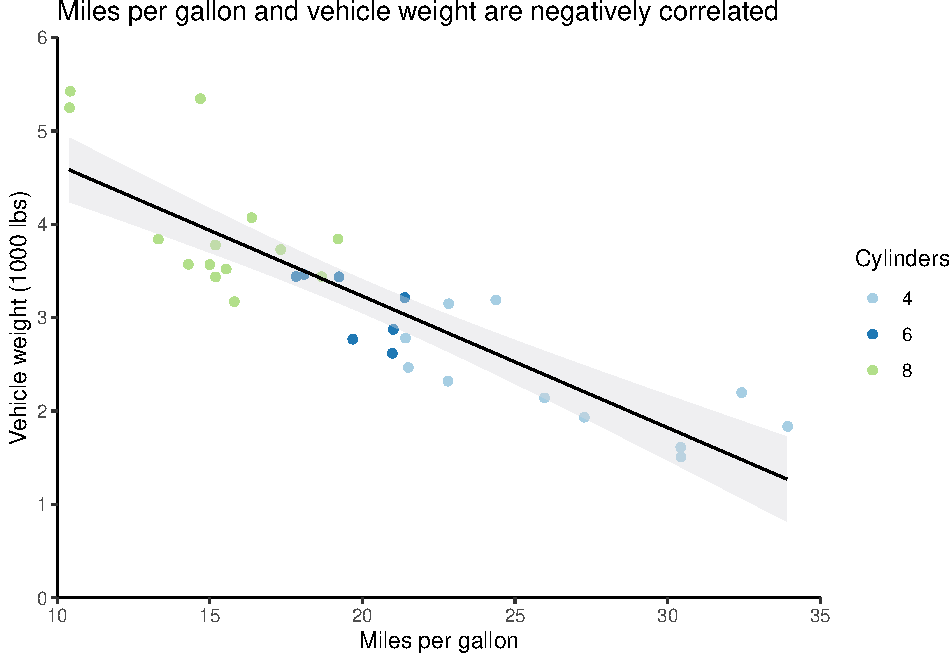
\includegraphics{rmarkdown-guide_files/figure-latex/content_graph_1-1.pdf}

You can use the chunk options to control how this graph appears in the document. The ones I typically use for outputting graphs are dots per inch (\texttt{dpi}) to control the image quality, \texttt{out.width} and \texttt{out.height} with either specific units or a percentage, and \texttt{fig.align} to change the alignment of the output. In the graph below, I've set \texttt{dpi} equal to 300, the \texttt{out.width} at 50\%, and \texttt{fig.align} to center. You can also add a figure caption in the chunk header if you'd like. These all go in the curly brackets at the top of the chunk and are separated by commas.

\begin{Shaded}
\begin{Highlighting}[]
\CommentTok{# Output plot with new chunk options}
\NormalTok{mtcars_scatter}
\end{Highlighting}
\end{Shaded}

\begin{center}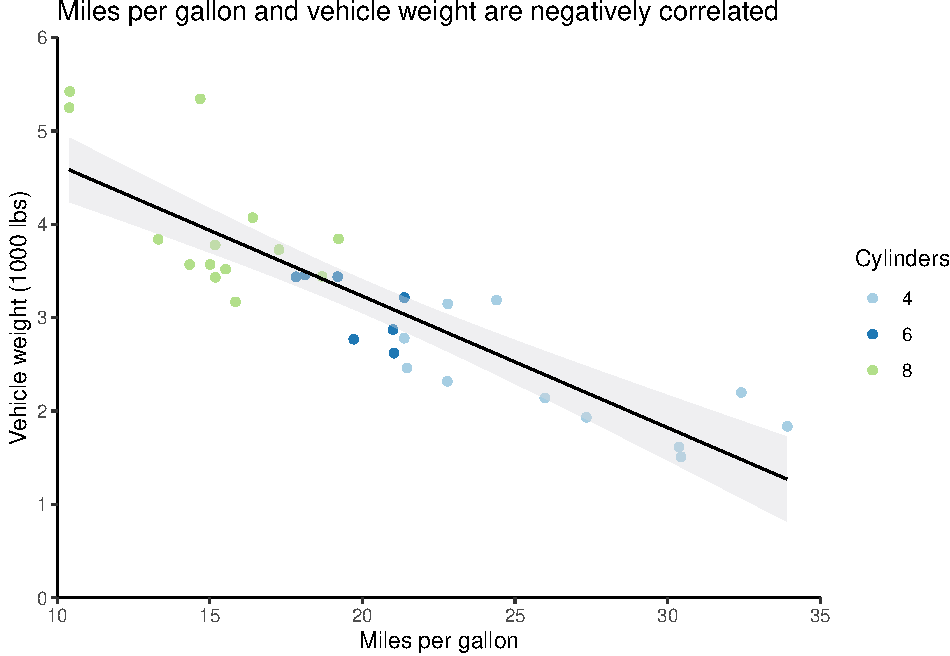
\includegraphics[width=0.5\linewidth]{rmarkdown-guide_files/figure-latex/content_graph_2-1} \end{center}

As a note, the values for \texttt{out.width} and \texttt{fig.align} need to be in quotation marks, while the value for the \texttt{dpi} setting doesn't. Pay attention to which values have quotes around them in the column with the default values in the chunk options section of the \href{https://rstudio.com/wp-content/uploads/2015/03/rmarkdown-reference.pdf}{reference guide}. You'll get an error when you try to render the document if you don't have appropriate quotation marks.

\hypertarget{tables}{%
\subsection{Tables}\label{tables}}

There are many ways to create tables in R. My preferred way is with \texttt{knitr::kable} and \texttt{kableExtra}. Together these allow you to create ``complex tables and manipulate table styles'' as the \href{https://cran.r-project.org/web/packages/kableExtra/vignettes/awesome_table_in_html.html}{documentation} says. You use the pipe operator \texttt{\%\textgreater{}\%} from \texttt{magrittr} the way you use the plus sign for \texttt{ggplot} to add layers of formatting. If you don't specify the output format, \texttt{knitr} will automatically create an HTML table for you unless you're rendering to a PDF when it will use LaTeX. You can override this locally in \texttt{kable} or globally with \texttt{knitr::options}.

\begin{Shaded}
\begin{Highlighting}[]
\CommentTok{# Get coefficients table from mpg_summary}
\NormalTok{mpg_coefs <-}\StringTok{ }\NormalTok{mpg_summary}\OperatorTok{$}\NormalTok{coefficients}

\CommentTok{# Create minimal table}
  \CommentTok{# Pass table to kable, then format with kable_styling}
\NormalTok{mpg_coefs }\OperatorTok
\StringTok{  }\KeywordTok{kable}\NormalTok{() }\OperatorTok
\StringTok{  }\KeywordTok{kable_styling}\NormalTok{()}
\end{Highlighting}
\end{Shaded}

\begin{table}[H]
\centering
\begin{tabular}{l|r|r|r|r}
\hline
  & Estimate & Std. Error & t value & Pr(>|t|)\\
\hline
(Intercept) & 37.285126 & 1.877627 & 19.857575 & 0\\
\hline
wt & -5.344472 & 0.559101 & -9.559044 & 0\\
\hline
\end{tabular}
\end{table}

This is obviously a very minimal table. The documentation for HTML and LaTeX tables is great, so if you're looking for something in particular it will be relatively easy for you to find. I have a more complex example in Section \ref{csshtml}, to which I added custom CSS code, among other things. You can see what the output of that code would look like in my \href{https://github.com/hollzzar/psychonomics-poster/blob/master/Psychonomics.pdf}{Psychonomics poster}.

\hypertarget{images}{%
\subsection{Images}\label{images}}

It's very easy to embed images. You've already seen this in Section \ref{chunkex}. Just use the \texttt{knitr::include\_graphics} function, and you can control the output as you would for a graph by specifying the chunk options. You can also use CSS or \texttt{!{[}caption{]}(file/path)} notation, but I find the chunk approach to be more straight-forward.

When I have very complex graphs that take a long time to render, or graphs that don't play very nicely with R Markdown (like those from \texttt{corrplot}), I'll save them as images and include them this way.

I also save graphs as images first when I need to crop them to maintain the correct aspect ratio. This is true of the participant maps I created for my \href{https://github.com/hollzzar/psychonomics-poster/blob/master/Psychonomics.pdf}{Psychonomics} and \href{https://github.com/hollzzar/CNS-2020-poster/blob/master/CNS_2020.pdf}{CNS} posters. Instead of using \texttt{knitr::include\_graphics}, I use \texttt{image\_read} from the \texttt{magick} package to load the image, followed by the \texttt{image\_trim} function (you can't go straight from a \texttt{ggplot} graph to these functions).

\hypertarget{rintext}{%
\section{Inline R}\label{rintext}}

A very useful aspect of R Markdown is that you can call R objects and functions in markdown or the YAML header by sandwiching them between backticks. For example, let's say I want to report on the names of the flower species in the \href{https://archive.ics.uci.edu/ml/datasets/iris}{\texttt{iris} dataset}.

\begin{Shaded}
\begin{Highlighting}[]
\CommentTok{# Pull species column from iris and get unique values in column}
\NormalTok{species <-}\StringTok{ }\NormalTok{iris }\OperatorTok\StringTok{ }\KeywordTok{pull}\NormalTok{(Species) }\OperatorTok\StringTok{ }\KeywordTok{unique}\NormalTok{()}

\CommentTok{# Print species variable}
\KeywordTok{print}\NormalTok{(species)}
\end{Highlighting}
\end{Shaded}

\begin{verbatim}
## [1] setosa     versicolor virginica 
## Levels: setosa versicolor virginica
\end{verbatim}

Maybe I also want to save a variable with the number of species in this list.

\begin{Shaded}
\begin{Highlighting}[]
\CommentTok{# Get number of unique species}
\NormalTok{species_count <-}\StringTok{ }\KeywordTok{length}\NormalTok{(species)}

\CommentTok{# Print number of species}
\KeywordTok{print}\NormalTok{(species_count)}
\end{Highlighting}
\end{Shaded}

\begin{verbatim}
## [1] 3
\end{verbatim}

I can call \texttt{species} and \texttt{species\_count} in the markdown text to reference these variables dynamically. Just as in a code chunk, I have to specify that I'm working with R code by including a lower-case r in the backticks with the variable.

So if I put ``r species\_count'' between backticks, I can report that there are 3 species without typing out the number itself. Or I can reference the variable with the exact species names: setosa, versicolor, virginica. You can see what the markdown looks like in the screenshot below.


\includegraphics[width=22.67in]{images/content_intext_iris}

You'll also note that \texttt{knitr} automatically put commas between the species names. To be honest, this is an aspect of R Markdown that I don't explore very much. I tend to format the variables exactly how I want them to appear in the text before referencing them with inline code. If I find a good explanation of this behavior, I'll link to it here.

\hypertarget{format}{%
\chapter{Formatting}\label{format}}

There are many ways to customize the formatting of an R Markdown document. In the YAML header, you can specify different parameter options or reference external documents. You can also edit templates directly in certain cases. For local formatting, you can include inline code in the markdown sections.

\hypertarget{yaml-parameters}{%
\section{YAML parameters}\label{yaml-parameters}}

There are several \href{https://ymlthis.r-lib.org/articles/yaml-fieldguide.html}{general YAML options} that you can include in the YAML header to format your documents. You can also add \textbf{params} to the YAML header that you can specify when you render your document and call in your code chunks to make \href{https://rmarkdown.rstudio.com/developer_parameterized_reports.html\%23parameter_types\%2F}{parameterized reports}. Some YAML options require quotation marks, while others don't. In general, if the YAML option is a string of text that you're specifying, like the title or your name, then it should be in quotes. If you're setting a programmatic option, like the output type, then it shouldn't be in quotes.

For the string options, there's some custom formatting you can do. The first example below shows how you can center a title and force a line break. The second shows how you can automatically pull the date and time when you knit your document and format it in a particular way. This is actually R code that is embedded in a string by putting the function call between backticks with a lowercase r. You can use the same principle to put R code and functions in the text of an R Markdown document, as described in Section \ref{rintext}.

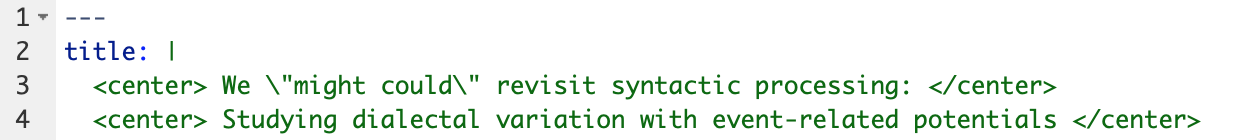
\includegraphics[width=17.36in]{images/formatting_title}
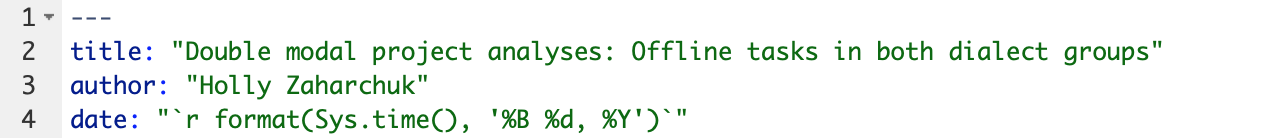
\includegraphics[width=17.69in]{images/formatting_date}

\begin{Shaded}
\begin{Highlighting}[]
\CommentTok{# Show date formatting code}
  \CommentTok{# You can run ?Sys.time in the console for more information }
  \CommentTok{# on the options you can pass to format}
\KeywordTok{format}\NormalTok{(}\KeywordTok{Sys.time}\NormalTok{(), }\StringTok{'%B %d, %Y'}\NormalTok{)}
\end{Highlighting}
\end{Shaded}

\begin{verbatim}
## [1] "May 04, 2020"
\end{verbatim}

There are also template-specific parameters, but you'll need to look at the specific package documentation to know what these are.

\hypertarget{yamlref}{%
\section{YAML references}\label{yamlref}}

In your YAML header, you can reference other documents for formatting and content.

\hypertarget{bib}{%
\subsection{.bib}\label{bib}}

To cite references, you need to set the \emph{bibliography} option in the YAML header. I use \href{https://bibdesk.sourceforge.io/}{BibDesk} for my reference manager, which creates a .bib file, or you can create a .bib file directly in LaTeX. You can also construct a \href{https://rmarkdown.rstudio.com/authoring_bibliographies_and_citations.html}{.bib file} through R. See Section \ref{scholarex} or the \href{https://github.com/hollzzar/zaharchuk-cv/blob/master/Zaharchuk_CV.Rmd}{.Rmd file for my CV} for examples with the \texttt{scholar} package.

By default, if you reference a .bib file, the references will appear at the very end of the document. This is usually fine, but sometimes you may want to control the placement of the references, as with a CV. In this case, you can use a .lua filter as described in Section \ref{luaex} to place your references in a particular spot.

To create in-text citations, you'll use the cite key from your .bib file with the @ symbol. Full information on citing syntax can be found \href{https://rmarkdown.rstudio.com/authoring_bibliographies_and_citations.html\#citation_syntax}{here}. When you cite something from your .bib file, it will appear in your references section when you knit your document. If you want to include all of the references from your .bib file in your reference section, regardless of whether you've cited them or not in the document, set the \textbf{nocite} option in the YAML header to \textbf{``@*''}.

\hypertarget{csl}{%
\subsection{.csl}\label{csl}}

To determine the type of formatting for your references, you can include a citation style language or \href{https://github.com/citation-style-language/styles}{.csl file}. There are other ways to set the format of bibliographies, but a .csl file allows fine-grained control over citations that you can also customize. My \href{https://github.com/hollzzar/zaharchuk-cv}{CV} repository has a customized APA 6 .csl file for arranging references in descending order by date. My \href{https://github.com/hollzzar/psychonomics-poster}{Psychonomics poster} repository also has a customized APA 6 .csl to fix some small bugs.

\hypertarget{cls-and-.css}{%
\subsection{.cls and .css}\label{cls-and-.css}}

You can include .cls files (not to be confused with the .csl files above) for LaTeX styling or .css files for HTML styling. You can see an example of the .cls file that formats my \href{https://github.com/hollzzar/zaharchuk-cv}{CV} in Section \ref{clsex}. This guide itself uses .css files that you can find \href{https://github.com/hollzzar/rmarkdown-guide}{here} to control the formatting.

\hypertarget{luaex}{%
\subsection{.lua}\label{luaex}}

Sometimes, you need to interact with pandoc directly in order to achieve a particular formatting outcome. To do this, you need to use a .lua filter.

The \href{https://github.com/pandoc/lua-filters/tree/master/multiple-bibliographies}{multiple-bibliographies.lua file} is incredibly useful. It allows you to use multiple bibliographies in one document, as I do in my \href{https://github.com/hollzzar/zaharchuk-cv}{CV} (one for publications, another for conference presentations). Even if you don't have multiple bibliographies, using this .lua filter will allow you to place your reference section in a particular part of your document.

The \href{https://github.com/hollzzar/zaharchuk-cv/blob/master/Zaharchuk_CV.Rmd}{.Rmd file for my CV} shows how to use multiple bibliographies in R Markdown. First, you need to add a name to each bibliography in the YAML header with an underscore. You can also see how I've referenced this .lua file in the \textbf{pandoc\_args} option in the YAML header. For this document to knit properly, the .lua file needs to be in the same place as my .Rmd file.

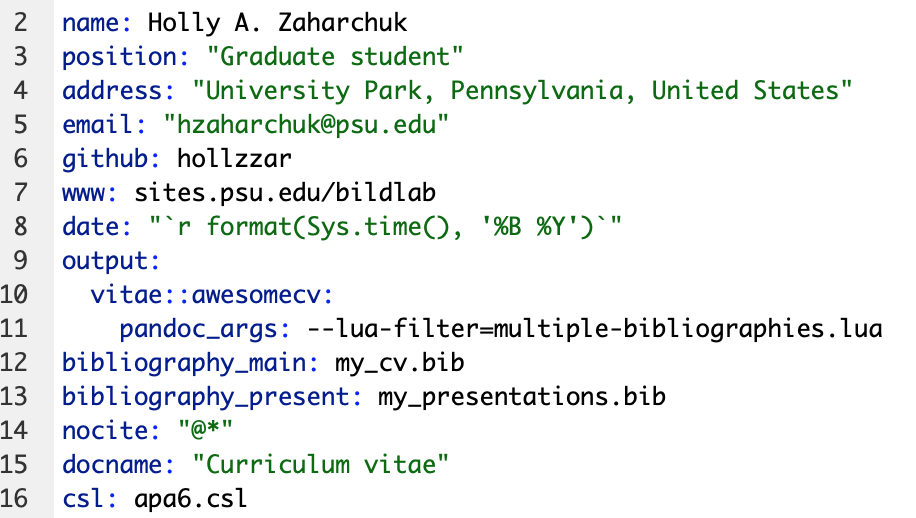
\includegraphics[width=12.72in]{images/references_example}

Then, you can place the reference section for each bibliography in the appropriate place. This example also shows how you can alter the formatting locally for just the reference section with LaTeX commands.

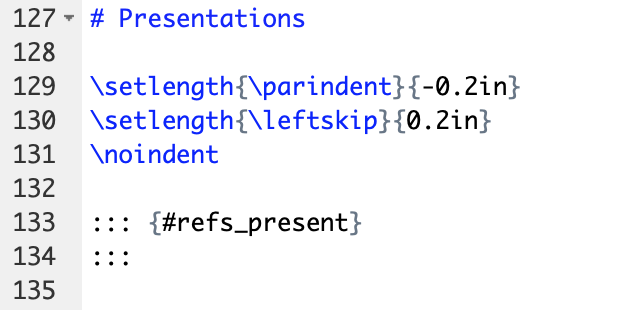
\includegraphics[width=8.64in]{images/references_placement}

Another very useful .lua file handles in-text APA citations. By default, pandoc uses ``\&'' for in-text citations where APA would require ``and,'' even if you're using a .csl file for APA formatting. Rather than downloading a file like \emph{multiple-bibliographies.lua}, this file is already stored with pandoc: you just need to reference it. Follow \href{https://cran.rstudio.com/web/packages/rmdfiltr/vignettes/replace_ampersands.html}{these instructions} to access and reference this .lua filter The example below from my Master's thesis shows how you can reference multiple .lua filters in one document.

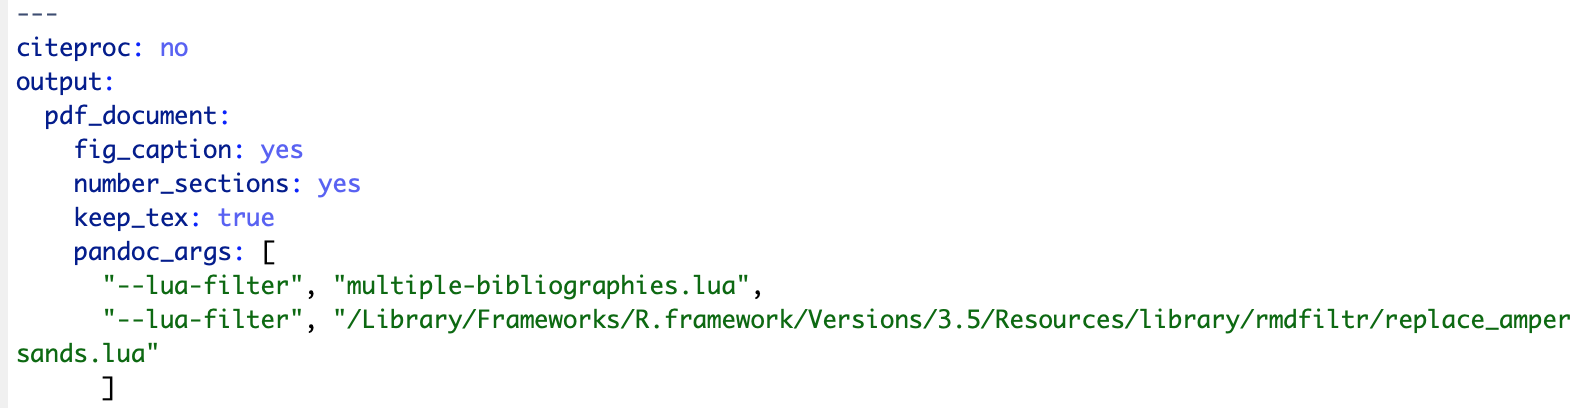
\includegraphics[width=21.94in]{images/lua_example}

\hypertarget{editing-templates}{%
\section{Editing templates}\label{editing-templates}}

To make extremely custom edits to templates, sometimes you have to edit the template documents directly. If the template generates a style document (e.g., .cls) in the directory with your .Rmd file, you can usually edit that without going to the package. Otherwise, you have to find out where your computer stores your R packages and edit the template there.

\hypertarget{clsex}{%
\subsection{Directory documents}\label{clsex}}

Some templates output formatting documents in your working directory. These are easier to access and edit. For example, knitting the \texttt{vitae::awesomecv} template created a .cls file that I could edit to change font sizes/colors.

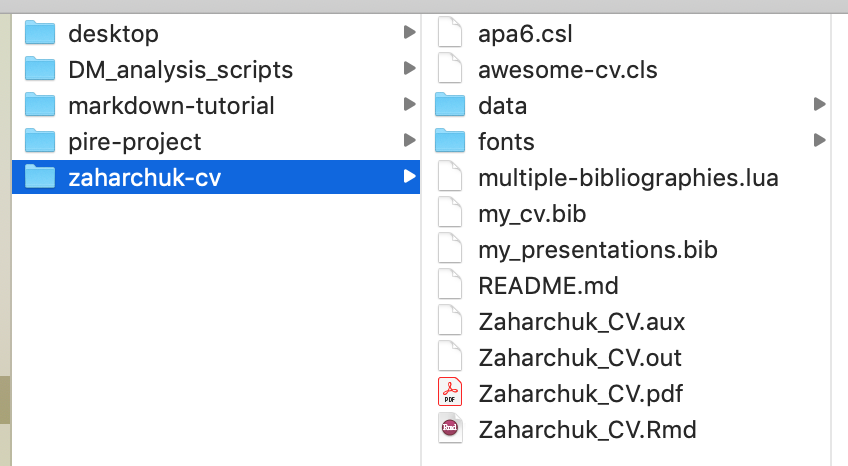
\includegraphics[width=11.78in]{images/template_dir}

\hypertarget{package-documents}{%
\subsection{Package documents}\label{package-documents}}

To find out where your packages ``live,'' you can call \texttt{installed.packages}. When you leave the parentheses blank (i.e., if you don't provide any arguments), as I've done below, the function will return all of the packages you have installed. I've stored them as a dataframe, and then filtered for an example. Here, I'm looking at the \texttt{posterdown} package.

\begin{Shaded}
\begin{Highlighting}[]
\CommentTok{# Make dataframe with installed packages}
\NormalTok{pkgs <-}\StringTok{ }\KeywordTok{installed.packages}\NormalTok{() }\OperatorTok
\StringTok{  }\KeywordTok{as.data.frame}\NormalTok{()}

\CommentTok{# Pull posterdown package }
\NormalTok{pstr <-}\StringTok{ }\NormalTok{pkgs }\OperatorTok\StringTok{ }
\StringTok{  }\KeywordTok{select}\NormalTok{(Package, LibPath, Version, Depends, Imports) }\OperatorTok
\StringTok{  }\NormalTok{dplyr}\OperatorTok{::}\KeywordTok{filter}\NormalTok{(Package }\OperatorTok{==}\StringTok{ "posterdown"}\NormalTok{)}

\CommentTok{# Make table}
\KeywordTok{kable}\NormalTok{(pstr) }\OperatorTok
\StringTok{  }\KeywordTok{kable_styling}\NormalTok{(}\DataTypeTok{bootstrap_options =} \StringTok{"condensed"}\NormalTok{, }\DataTypeTok{full_width =} \OtherTok{FALSE}\NormalTok{, }\DataTypeTok{font_size =} \DecValTok{12}\NormalTok{)}
\end{Highlighting}
\end{Shaded}

\begin{table}[H]
\centering\begingroup\fontsize{12}{14}\selectfont

\begin{tabular}{l|l|l|l|l}
\hline
Package & LibPath & Version & Depends & Imports\\
\hline
posterdown & /Library/Frameworks/R.framework/Versions/3.5/Resources/library & 1.0 & NA & pagedown, rmarkdown, yaml\\
\hline
\end{tabular}
\endgroup{}
\end{table}

To edit package documents once you've located them, you should proceed with caution. Be sure to:

\begin{itemize}
\tightlist
\item
  Save the original template and move it to a different location (in the example below, I made the ``original'' folder and put the original template there)
\item
  Make one change at a time, and then re-knit the document to see what changed
\item
  Name the updated template with the same name in the same place as the original (here, in the ``resources'' folder)
\end{itemize}

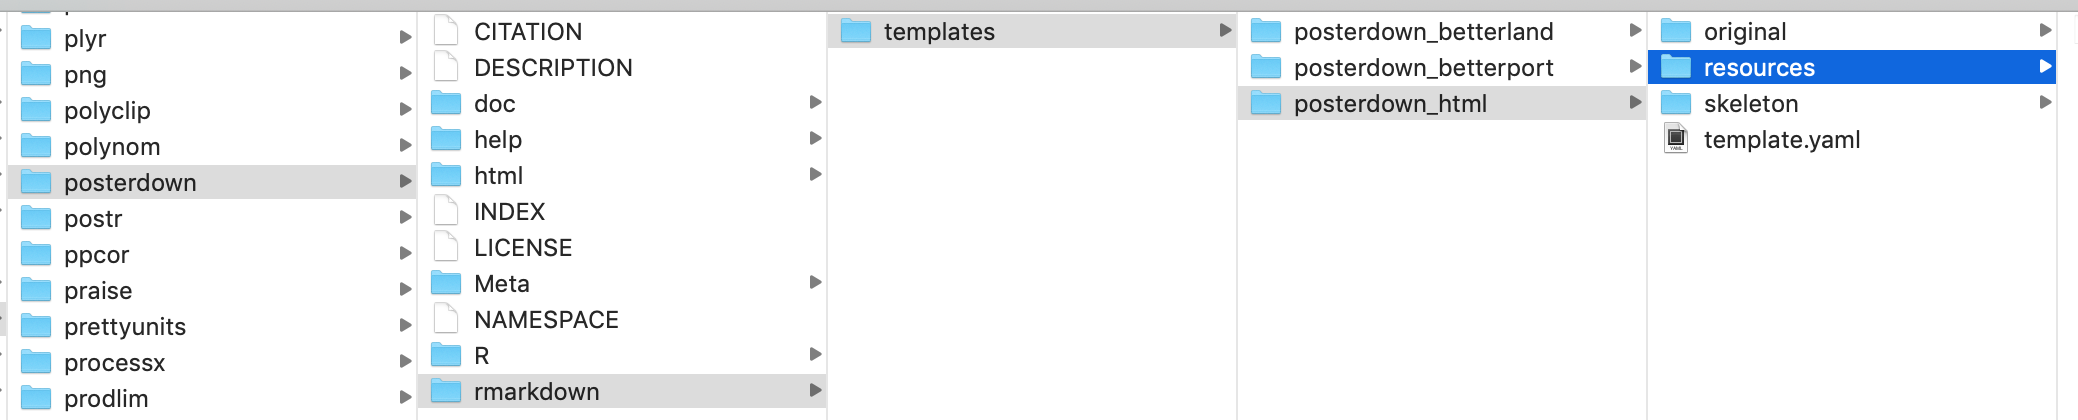
\includegraphics[width=28.86in]{images/template_package}

\hypertarget{inline-code}{%
\section{Inline code}\label{inline-code}}

R Markdown supports inline code for custom formatting.

\hypertarget{latexpacks}{%
\subsection{LaTeX}\label{latexpacks}}

In PDFs, you can use code, typesetting commands (e.g., \textbackslash vspace\{12pt\}), and specific packages from LaTeX. There are useful lists of symbols \href{https://www.rpi.edu/dept/arc/training/latex/LaTeX_symbols.pdf}{here} and \href{https://www.tug.org/tugboat/tb17-2/tb51rei.pdf}{here}. Check out \href{https://www.rosannavanhespen.nl/thesis_in_rmarkdown/}{Writing Your Thesis with R Markdown} and Section \ref{latexpacks} below for examples using LaTeX packages and typesetting commands.

I've included examples of calling packages in the YAML header and using inline functions from my statistics homework below.

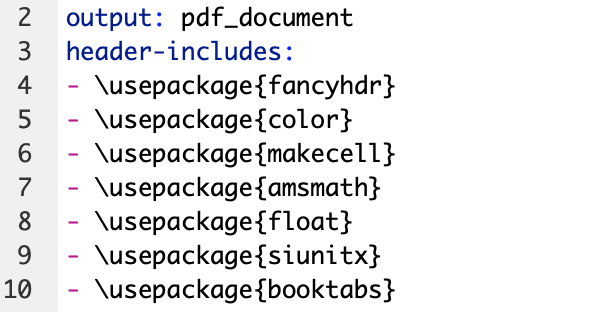
\includegraphics[width=8.31in]{images/latex_packages}

\includegraphics[width=9.31in]{images/latex_calls}


\includegraphics[width=18.97in]{images/latex_example}

\hypertarget{csshtml}{%
\subsection{CSS/HTML}\label{csshtml}}

In HTML documents, you can include \href{https://developer.mozilla.org/en-US/docs/Web/CSS}{CSS} commands. I have some examples in \href{https://github.com/hollzzar/markdown-tutorial/blob/master/brownbag_slides.Rmd}{these \texttt{revealjs} slides}, where I wanted to left-align slide text while keeping titles centered.

Here are some examples of using CSS from my \href{https://github.com/hollzzar/psychonomics-poster/blob/master/Psychonomics.Rmd}{Psychonomics poster}. The first example includes custom CSS in a \texttt{knitr::kable} table to add borders of a particular color between some rows. The second example changes the font size of the references section at the end of the poster.

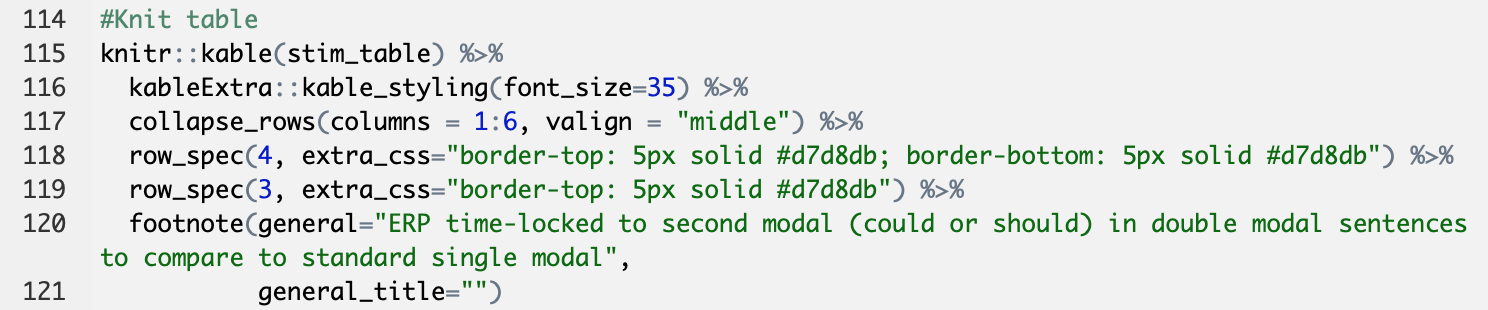
\includegraphics[width=20.67in]{images/css_example}

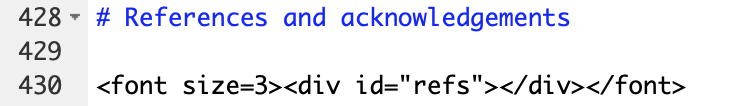
\includegraphics[width=10.39in]{images/html_example}

\hypertarget{help}{%
\section{Custom functions}\label{help}}

If you're fairly comfortable with R, you can write formatting functions for yourself to make your life easier when you're referencing variables in your text.

When I was working on my Master's thesis, I wrote some custom functions for statistical values that I had to report over and over. This was particularly useful when I had to switch from referring to any \emph{p} values over .05 as \emph{p} \textgreater{} .05 to \emph{p} = the exact value. I just had to change the one function by commenting out a couple lines and re-knit my document. The function is included below; this was the most complicated of the ones I wrote, which included degrees of freedom, \emph{t} and \emph{F} values, reaction times, and percentages.

\begin{Shaded}
\begin{Highlighting}[]
\CommentTok{# Make number formatting function for p values}
\CommentTok{# val is the p value I want to format}
\CommentTok{# format_code specifies whether I want to include the symbol or not}
  \CommentTok{# format_code defaults to including the symbol}
\NormalTok{p_formatting <-}\StringTok{ }\ControlFlowTok{function}\NormalTok{(val, }\DataTypeTok{format_code =} \DecValTok{1}\NormalTok{) \{}
  
  \CommentTok{# If I want to include the symbol (when I'm calling this variable in text)}
  \ControlFlowTok{if}\NormalTok{ (format_code }\OperatorTok{==}\StringTok{ }\DecValTok{1}\NormalTok{) \{}
    
    \CommentTok{# If the p value is less than .001, get the less than symbol}
      \CommentTok{# Otherwise, get the equals symbol}
      \CommentTok{# The next line, which I commented out for my thesis,}
      \CommentTok{# looks to see if the value was greater than .05}
\NormalTok{    sign_type <-}\StringTok{ }\KeywordTok{if_else}\NormalTok{(val }\OperatorTok{<}\StringTok{ }\FloatTok{0.001}\NormalTok{, }\StringTok{"<"}\NormalTok{, }\StringTok{"="}\NormalTok{)}
\NormalTok{    sign_type <-}\StringTok{ }\KeywordTok{if_else}\NormalTok{(val }\OperatorTok{>}\StringTok{ }\FloatTok{0.05}\NormalTok{, }\StringTok{">"}\NormalTok{, sign_type)}
    
    \CommentTok{# If the p value is less than .001, set the value equal to .001}
    \ControlFlowTok{if}\NormalTok{ (sign_type }\OperatorTok{==}\StringTok{ "<"}\NormalTok{) \{}
\NormalTok{      val <-}\StringTok{ ".001"}
      
    \CommentTok{# If the p value is greater than .05, set the value equal to .05 }
      \CommentTok{# I commented out these next two lines for my thesis}
\NormalTok{    \} }\ControlFlowTok{else} \ControlFlowTok{if}\NormalTok{ (sign_type }\OperatorTok{==}\StringTok{ ">"}\NormalTok{) \{}
\NormalTok{      val <-}\StringTok{ ".05"}
      
    \CommentTok{# Otherwise, get the actual p value,}
      \CommentTok{# round it to three decimal places, and}
      \CommentTok{# remove the leading zero}
\NormalTok{    \} }\ControlFlowTok{else}\NormalTok{ \{}
\NormalTok{      val <-}\StringTok{ }\KeywordTok{sprintf}\NormalTok{(}\StringTok{"%.3f"}\NormalTok{, val)}
\NormalTok{      val <-}\StringTok{ }\KeywordTok{substring}\NormalTok{(val, }\DecValTok{2}\NormalTok{)}
\NormalTok{    \}}
    
    \CommentTok{# Combine the new/formatted p value with >, <, or =,}
      \CommentTok{# depending on the p value}
\NormalTok{    val_string <-}\StringTok{ }\KeywordTok{paste}\NormalTok{(sign_type, val, }\DataTypeTok{sep =} \StringTok{" "}\NormalTok{)}
\NormalTok{    val_string}
  
  \CommentTok{# If I don't want the symbol (as in a table),}
    \CommentTok{# just round the value to three decimal places}
    \CommentTok{# and remove the leading zero}
\NormalTok{  \} }\ControlFlowTok{else} \ControlFlowTok{if}\NormalTok{ (format_code }\OperatorTok{==}\StringTok{ }\DecValTok{0}\NormalTok{) \{}
    
\NormalTok{    val <-}\StringTok{ }\KeywordTok{sprintf}\NormalTok{(}\StringTok{"%.3f"}\NormalTok{, val)}
\NormalTok{    val_string <-}\StringTok{ }\KeywordTok{substring}\NormalTok{(val, }\DecValTok{2}\NormalTok{)}
\NormalTok{    val_string}
    
\NormalTok{  \}}
  
\NormalTok{\}}
\end{Highlighting}
\end{Shaded}

I've included an example with this function below to demonstrate how you can really streamline your analysis-to-presentation pipeline with a simple function.

\begin{Shaded}
\begin{Highlighting}[]
\CommentTok{# Create arbitrary p value}
\NormalTok{p_value <-}\StringTok{ }\FloatTok{0.0123}

\CommentTok{# Format p value including symbol}
\NormalTok{p_value_}\DecValTok{1}\NormalTok{ <-}\StringTok{ }\KeywordTok{p_formatting}\NormalTok{(p_value)}

\CommentTok{# Format p value not including symbol}
\NormalTok{p_value_}\DecValTok{0}\NormalTok{ <-}\StringTok{ }\KeywordTok{p_formatting}\NormalTok{(p_value, }\DataTypeTok{format_code =} \DecValTok{0}\NormalTok{)}
\end{Highlighting}
\end{Shaded}

Here is the original \emph{p} value: 0.0123. I can write \emph{p} = .012 to reference the variable that already has the symbol, or I can reference the variable without the symbol: .012. I've included an image of these lines below to give you a sense of how this looks in markdown.

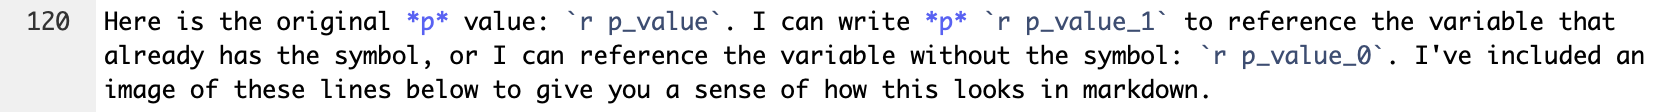
\includegraphics[width=23.06in]{images/content_intext}

\hypertarget{organization}{%
\chapter{Organization}\label{organization}}

If you're working on a large R Markdown project, like a thesis, it's inevitable that you will have several code chunks to perform pieces of one process (e.g., reformatting data for plotting and then creating the plots), and you will have lots of chapters/sections of markdown.

At a minimum, you want to keep your chunks small and name them for easy troubleshooting and use headers at multiple levels. One thing to note is that you cannot have the same chunk names anywhere in your document or sub-documents; this will throw an error. If you go to the bottom left-hand corner of your .Rmd file in RStudio, you'll see a small drop-down menu. There, you can jump to specific headers and code chunks.

As your documents grow, however, even these sections will become difficult to keep straight. This is when you want to use what are called \emph{child} documents. This just means that you have separate R Markdown documents that you reference in your main R Markdown document. These are also great if you need to include the same code or text in multiple documents.

\hypertarget{child-documents}{%
\section{\texorpdfstring{\texttt{child} documents}{child documents}}\label{child-documents}}

The screenshot below shows some code from my main Master's thesis R Markdown document. In this example, I referenced another R Markdown document called \emph{Load}, as well as one called \emph{chapter1}. All you have to do is make a code chunk in which you set the \texttt{child} parameter equal to the file that you want to reference (and file path if it's in a subfolder, as I have here). The chunk itself must be empty.

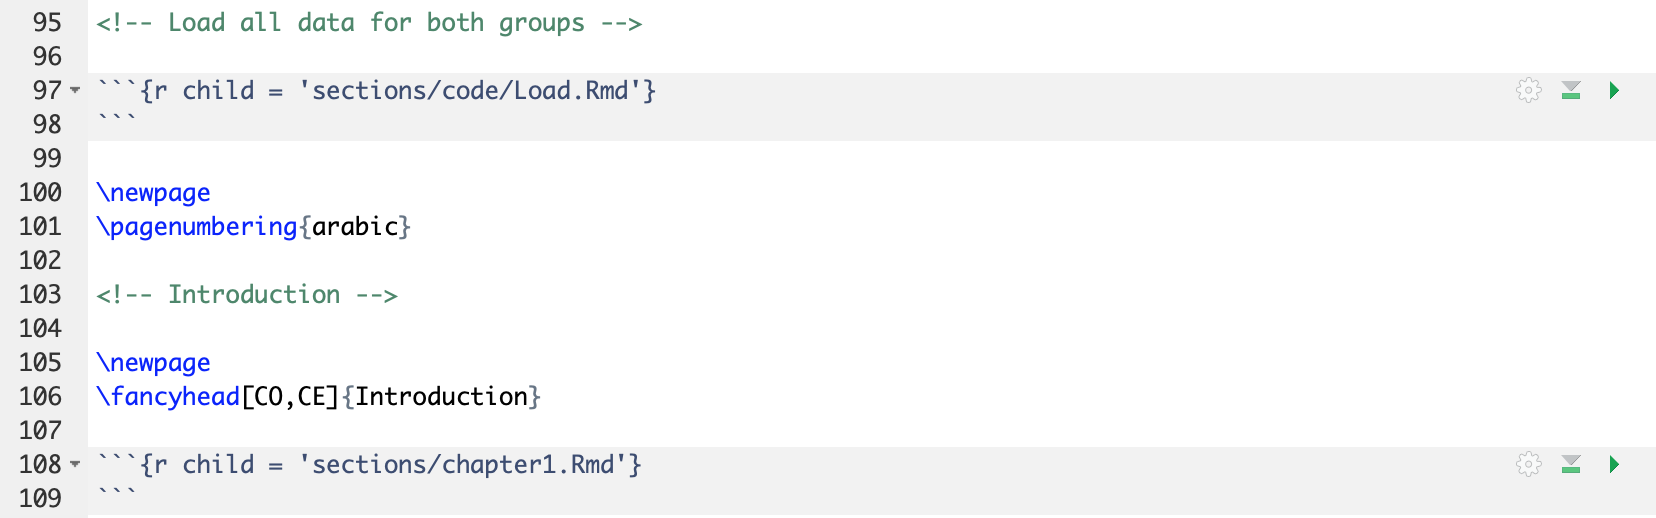
\includegraphics[width=23in]{images/content_child_call}

The \emph{Load} document contained several code chunks for loading and processing my data and analyses for presentation. I've included a screenshot of the top of this document below. You can see that I just gave it a \textbf{pagetitle} in the YAML header, and then included the code chunks that I wanted. This helped keep the main document uncluttered.

One thing to note is that when you're running your code chunks to work on your document, if you just run the code chunk referencing the \texttt{child} document, nothing will happen. You have to open that R Markdown document and run it to evaluate those chunks.

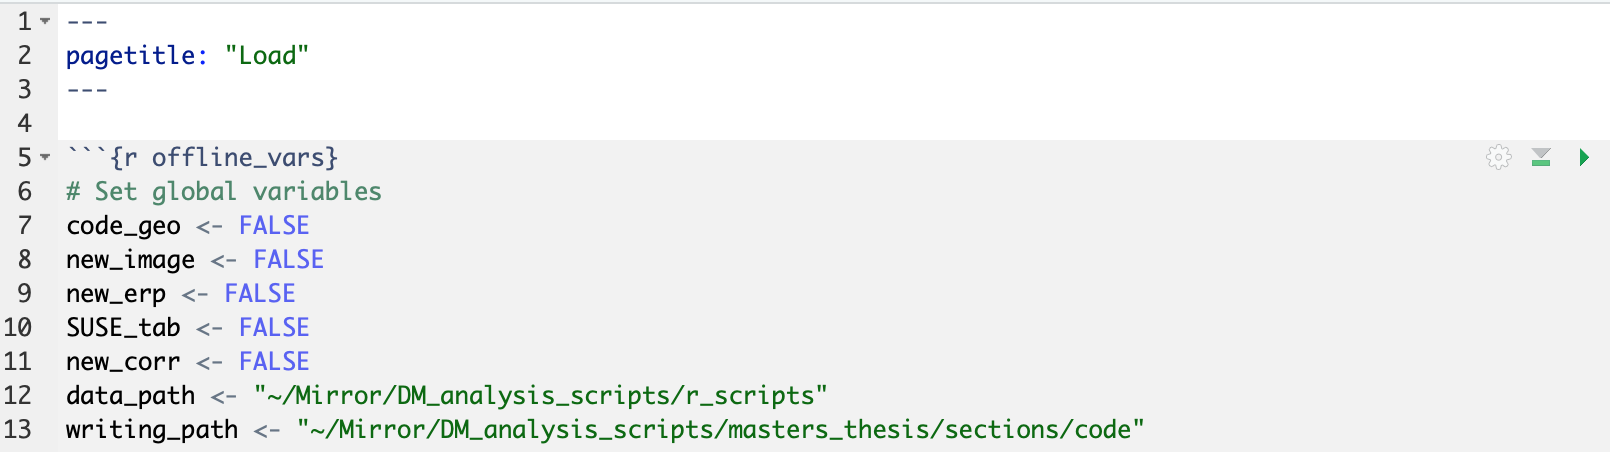
\includegraphics[width=22.36in]{images/content_child_setup}

You also saw that I loaded the \emph{chapter1} \texttt{child} document. This allowed me to separate out each of the sections of my thesis into different documents, in addition to separating out the analyses as with the \emph{Load} document. I organized these documents into subfolders to keep everything clean. I've included a screenshot of the organizational structure below.

At the top level, I had the main R Markdown document and necessary reference documents (see Section \ref{yamlref} for more information on including reference documents in the YAML header). In the first subfolder, I had the documents for each section of the thesis (e.g., \emph{chapter1} is the introduction). In the lower subfolder, I had documents that only contained code chunks (e.g., running statistical analyses and formatting the values for referencing).

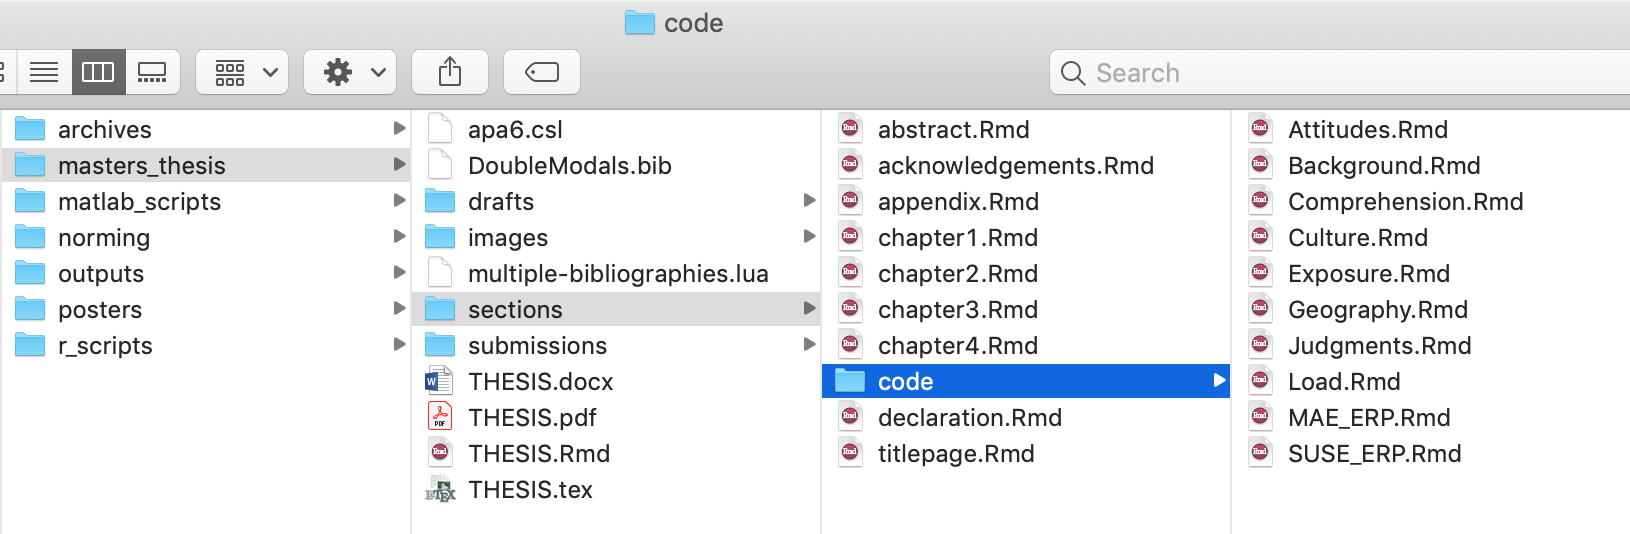
\includegraphics[width=22.64in]{images/content_organization}

\hypertarget{source}{%
\section{Sourcing code}\label{source}}

I also use a similar decentralized organizational structure for my actual R processing scripts. You can use \texttt{source} to import all of the code from one script into another, similarly to using \texttt{child} documents in R Markdown. The \emph{Load} document above actually uses code chunks to load data from external R scripts into the thesis document.

I've included a screenshot of the folder with all of my R scripts for preparing my thesis data. The data themselves are in the \emph{behavioral} and \emph{erp} subfolders. The \emph{DM\_global\_vars} file contains variables, like the custom formatting functions I described in Section \ref{help}, that I used across the scripts. I recommend having such a file that you \texttt{child} at the lowest level of the importing hierarchy. That way, if you need to change something, you can make that change in just one place.

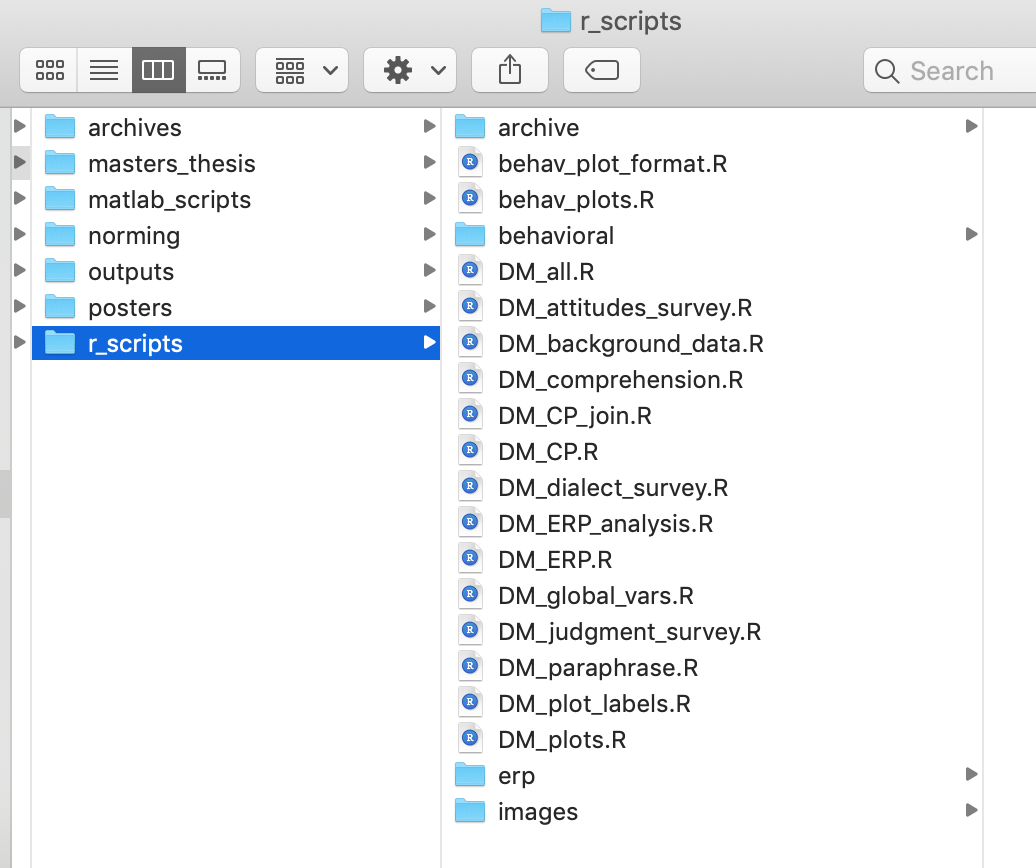
\includegraphics[width=14.39in]{images/content_organization_scripts}

\hypertarget{trouble}{%
\chapter{Troubleshooting}\label{trouble}}

\begin{enumerate}
\def\labelenumi{\arabic{enumi}.}
\tightlist
\item
  Warnings vs.~errors
\item
  RStudio vs.~R Markdown environments
\item
  Package issues
\item
  Strategies for troubleshooting issues
\end{enumerate}

\hypertarget{warnings-vs.-errors}{%
\section{Warnings vs.~errors}\label{warnings-vs.-errors}}

\hypertarget{warnings}{%
\subsection{Warnings}\label{warnings}}

Warnings won't stop your document from compiling, but generally indicate that you should change something in your code.

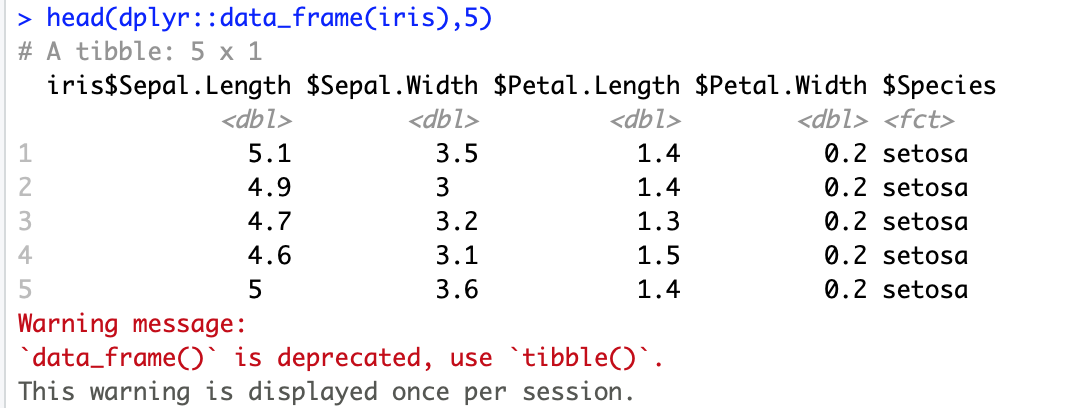
\includegraphics[width=14.92in]{images/warning_example}

\hypertarget{errors}{%
\subsection{Errors}\label{errors}}

There are different kinds of errors that you can encounter. In general, you can distinguish chunk errors from R Markdown errors by their appearance. Errors will usually tell you which line of the document they're in, but the line numbers can be misleading or inaccurate, so try to understand the error message first before going to look for the source. As always, Google and Stack Overflow are your friends!

Chunk error:

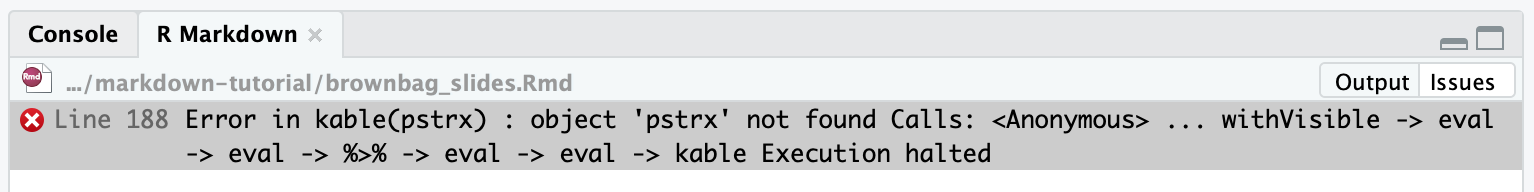
\includegraphics[width=21.31in]{images/error_example}

R Markdown error:


\includegraphics[width=21.33in]{images/error_conversion}

\hypertarget{environments}{%
\section{Environments}\label{environments}}

Running a chunk executes the code in the console and adds the output to your R environment; however, your R environment is separate from the environment created when knitting a document. When you render your document, it ignores your R environment. \texttt{knitr} runs all of the chunks in order and knits them into the markdown text.

If you're getting an error message that says a particular variable or package doesn't exist when it's loaded in your R environment, it's usually because you haven't included it in a previous chunk.

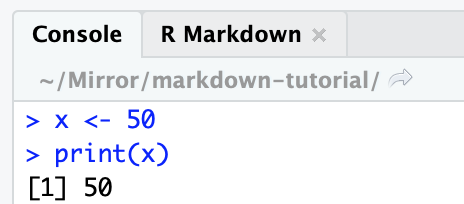
\includegraphics[width=6.44in]{images/environment_console}
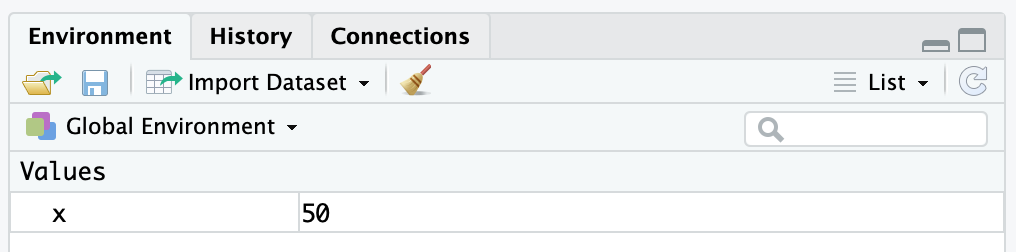
\includegraphics[width=14.11in]{images/environment_var}

\begin{Shaded}
\begin{Highlighting}[]
\CommentTok{# Define new variable y}
\NormalTok{y <-}\StringTok{ }\DecValTok{100}

\CommentTok{# When I run this chunk, I get the expected output (150),}
\CommentTok{# but it fails when I try to knit the document}
\CommentTok{# I've set eval=FALSE for this chunk, so it doesn't try to run and prevent my document from knitting}
\KeywordTok{print}\NormalTok{(x }\OperatorTok{+}\StringTok{ }\NormalTok{y)}
\end{Highlighting}
\end{Shaded}

\hypertarget{package-issues}{%
\section{Package issues}\label{package-issues}}

\hypertarget{package-specification}{%
\subsection{Package specification}\label{package-specification}}

If a function you want to use isn't included in \texttt{base} R, you need to load the package that it's in. The most basic way to do this is to run \texttt{library(package)} for each individual package. As you saw in my ``setup'' chunk example in Section \ref{chunkex}, my preferred way is to set a list of packages and then load them with the \texttt{p\_load} function from the \texttt{pacman} package. This way, you can easily load multiple packages at once.

If you don't want to load a whole package, you can use this notation: \texttt{package::function}. This tells R which package to look in. You especially want to do this if there are what are called ``namespace conflicts,'' where multiple packages have the same function name. I often run into this issue with the \texttt{filter} function from \texttt{dplyr}, so I always specify \texttt{dplyr::filter} even if I've already loaded \texttt{dplyr}.

\hypertarget{updates}{%
\subsection{Updates}\label{updates}}

You may get warnings or errors related to packages being out of date or certain functions being ``deprecated.'' You may need to update packages and software that interact with R and R Markdown to get your code to run and documents to knit. Depending on the feature that is out of date, there are different strategies for updating.

\begin{itemize}
\tightlist
\item
  \href{https://tex.stackexchange.com/questions/55437/how-do-i-update-my-tex-distribution}{Update your TeX distribution} from the command line
\item
  Update all packages (including \texttt{rmarkdown}) in library with \texttt{update.packages(path)}
\item
  Update individual packages by reinstalling with \texttt{install.packages("package")}
\item
  Update R in the console with the \texttt{updateR} package
\item
  Redownload RStudio to update
\end{itemize}

\hypertarget{strategies}{%
\section{Strategies}\label{strategies}}

If you're running into any issues with rendering your document, here are some things you can try:

\begin{itemize}
\tightlist
\item
  Reset your R environment

  \begin{itemize}
  \tightlist
  \item
    Clear all variables by running \texttt{rm(ls\ =\ list())} in the console
  \item
    Restart your R environment with CTRL/(control + fn) + shift + F10
  \item
    Run all chunks individually \textbf{in order} before compiling to test code
  \end{itemize}
\item
  Search for information

  \begin{itemize}
  \tightlist
  \item
    Use Help window
  \item
    Search for package in console with \texttt{?package} or \texttt{??package}
  \item
    Google the error you're getting with the package or function you're trying to use
  \end{itemize}
\end{itemize}

\hypertarget{supplement}{%
\chapter{Supplementary materials}\label{supplement}}

\hypertarget{beginner-r}{%
\section{Beginner R}\label{beginner-r}}

\begin{itemize}
\tightlist
\item
  Basic R functionality
\item
  Reading in data
\item
  Tidy R philosophy
\item
  Manipulating data with \href{https://rstudio.com/wp-content/uploads/2015/02/data-wrangling-cheatsheet.pdf}{core \texttt{tidyr} functions}
\end{itemize}

\hypertarget{basic-r-functionality}{%
\subsection{Basic R functionality}\label{basic-r-functionality}}

\begin{itemize}
\tightlist
\item
  Variables
\item
  Functions
\item
  Operators
\end{itemize}

\hypertarget{variables}{%
\subsection{Variables}\label{variables}}

The way R stores your information will determine the kinds of functions/operators you can use

\begin{itemize}
\tightlist
\item
  Data: dataframes
\item
  Values: lists, vectors, matrices, etc.
\end{itemize}

\begin{Shaded}
\begin{Highlighting}[]
\CommentTok{# Variables can be numbers, strings, etc.}
\NormalTok{some_val <-}\StringTok{ }\DecValTok{200}
\NormalTok{other_val <-}\StringTok{ }\OtherTok{TRUE}

\CommentTok{# Variables can also be lists of numbers, strings, etc.}
\NormalTok{a_list <-}\StringTok{ }\KeywordTok{c}\NormalTok{(}\StringTok{"a"}\NormalTok{, }\StringTok{"b"}\NormalTok{, }\StringTok{"c"}\NormalTok{)}

\CommentTok{# We can also make dataframes (which are essentially special lists)}
\NormalTok{a_dataframe <-}\StringTok{ }\KeywordTok{tibble}\NormalTok{(}\DataTypeTok{column_1 =} \DecValTok{1}\OperatorTok{:}\DecValTok{3}\NormalTok{,}
                      \DataTypeTok{column_2 =}\NormalTok{ a_list)}
\end{Highlighting}
\end{Shaded}

\hypertarget{functions}{%
\subsection{Functions}\label{functions}}

Functions take a certain number and certain types of ``arguments''

\begin{itemize}
\tightlist
\item
  \texttt{base} R functions: part of downloading R
\item
  Packages: need to be installed, then loaded

  \begin{itemize}
  \tightlist
  \item
    \texttt{install.packages(package)} once (or to update package)
  \item
    \texttt{library(package)} every R session
  \end{itemize}
\end{itemize}

Use Help window or \texttt{?package} to check argument names, types, and defaults

\begin{itemize}
\tightlist
\item
  Named arguments without values are required (and user-defined)
\item
  Named arguments with values show defaults
\item
  Elipses mean that you can add other optional arguments
\end{itemize}

\begin{Shaded}
\begin{Highlighting}[]
\CommentTok{# file: required}
\CommentTok{# header = TRUE: default}
\CommentTok{# ...: other potential arguments, like stringsAsFactors = FALSE}
\KeywordTok{read.csv}\NormalTok{(file, }\DataTypeTok{header =} \OtherTok{TRUE}\NormalTok{, }\DataTypeTok{sep =} \StringTok{","}\NormalTok{, }\DataTypeTok{quote =} \StringTok{"}\CharTok{\textbackslash{}"}\StringTok{"}\NormalTok{,}
         \DataTypeTok{dec =} \StringTok{"."}\NormalTok{, }\DataTypeTok{fill =} \OtherTok{TRUE}\NormalTok{, }\DataTypeTok{comment.char =} \StringTok{""}\NormalTok{, ...)}
\end{Highlighting}
\end{Shaded}

\hypertarget{base-r}{%
\subsection{\texorpdfstring{\texttt{base} R}{base R}}\label{base-r}}

\begin{Shaded}
\begin{Highlighting}[]
\CommentTok{# base R function}
\CommentTok{# Count the number of rows in this dataframe}
\KeywordTok{nrow}\NormalTok{(a_dataframe)}
\end{Highlighting}
\end{Shaded}

\begin{verbatim}
## [1] 3
\end{verbatim}

\begin{Shaded}
\begin{Highlighting}[]
\CommentTok{# If I give nrow() too many arguments, it will throw an error}
\KeywordTok{nrow}\NormalTok{(a_dataframe, a_list)}
\end{Highlighting}
\end{Shaded}

\begin{Shaded}
\begin{Highlighting}[]
\CommentTok{# If I give it the wrong kind of argument, it will just return NULL}
\CommentTok{# Some functions won't run at all with wrong kind of argument}
\KeywordTok{nrow}\NormalTok{(a_list)}
\end{Highlighting}
\end{Shaded}

\begin{verbatim}
## NULL
\end{verbatim}

\hypertarget{scholarex}{%
\subsection{Packages}\label{scholarex}}

\begin{Shaded}
\begin{Highlighting}[]
\CommentTok{# scholar package }
\KeywordTok{library}\NormalTok{(scholar)}

\CommentTok{# get_publications function}
\CommentTok{# Pull publications from Google Scholar for Marie Curie}
\KeywordTok{get_publications}\NormalTok{(}\StringTok{"EmD_lTEAAAAJ&EmD_lTEAAAAJ&"}\NormalTok{) }\OperatorTok\StringTok{ }
\StringTok{  }\NormalTok{dplyr}\OperatorTok{::}\KeywordTok{filter}\NormalTok{(cites }\OperatorTok{>}\StringTok{ }\DecValTok{30}\NormalTok{) }\OperatorTok\StringTok{ }
\StringTok{  }\KeywordTok{distinct}\NormalTok{(title, }\DataTypeTok{.keep_all =} \OtherTok{TRUE}\NormalTok{) }\OperatorTok
\StringTok{  }\KeywordTok{select}\NormalTok{(author, title) }\OperatorTok
\StringTok{  }\KeywordTok{head}\NormalTok{(}\DecValTok{2}\NormalTok{) }\OperatorTok
\StringTok{  }\KeywordTok{kable}\NormalTok{()}
\end{Highlighting}
\end{Shaded}

\begin{tabular}{l|l}
\hline
author & title\\
\hline
P Curie, M Sklodowska-Curie & Sur une substance nouvelle radio-active, contenue dans la pechblende\\
\hline
E Curie & Madame Curie: a biography\\
\hline
\end{tabular}

\hypertarget{operators}{%
\subsection{Operators}\label{operators}}

\begin{itemize}
\tightlist
\item
  Relational: \textgreater, \textless, ==, !=, \textless=, \textgreater=

  \begin{itemize}
  \tightlist
  \item
    \texttt{is.na}, \texttt{exists}, etc. will return TRUE/FALSE values
  \item
    \texttt{grep}, \texttt{filter}, \texttt{str\_detect}, etc. use TRUE/FALSE values
  \end{itemize}
\item
  Logical: !, \&, \&\&, \textbar, \textbar\textbar{}
\item
  Arithmetic
\end{itemize}

\hypertarget{reading-in-data}{%
\subsection{Reading in data}\label{reading-in-data}}

General parameters for csv files

\begin{Shaded}
\begin{Highlighting}[]
\KeywordTok{read.csv}\NormalTok{(}\StringTok{"file_name.csv"}\NormalTok{, }
         \DataTypeTok{header =} \OtherTok{TRUE}\NormalTok{, }
         \DataTypeTok{stringsAsFactors =} \OtherTok{FALSE}\NormalTok{, }
         \DataTypeTok{check.names =} \OtherTok{FALSE}\NormalTok{, }
         \DataTypeTok{na.strings =} \StringTok{""}\NormalTok{)}
\end{Highlighting}
\end{Shaded}

Avoid special characters (including spaces) in file names, directories, and column headers!

\begin{itemize}
\tightlist
\item
  \texttt{readxl} package for Excel spreadsheets
\item
  APIs for direct access to online data

  \begin{itemize}
  \tightlist
  \item
    \texttt{qualtRics} package for Qualtrics data
  \item
    \texttt{ggmap} package for Google services (geolocation data)
  \end{itemize}
\item
  \texttt{read\_table} from \texttt{readr} package for text files
\end{itemize}

\hypertarget{tidy-r-philosophy}{%
\subsection{Tidy R philosophy}\label{tidy-r-philosophy}}

\begin{itemize}
\tightlist
\item
  One variable per column
\item
  One observation per row
\end{itemize}

\hypertarget{manipulating-data-with-tidyr}{%
\subsection{\texorpdfstring{Manipulating data with \texttt{tidyr}}{Manipulating data with tidyr}}\label{manipulating-data-with-tidyr}}

\begin{itemize}
\tightlist
\item
  \texttt{\%\textgreater{}\%}: pass the results of one function on to another
\item
  \texttt{select}: choose columns by name
\item
  \texttt{mutate}: add/change columns
\item
  \texttt{filter}: filter for (or out) rows
\item
  \texttt{group\_by} and \texttt{summarise}: perform operations on groups of data
\item
  \sout{\mbox{\texttt{gather}} and \mbox{\texttt{spread}}} \texttt{pivot\_longer} and \texttt{pivot\_wider}: condense multiple columns into one or the inverse
\item
  \texttt{separate} and \texttt{unite}: split a column into multiple or the inverse
\end{itemize}

\hypertarget{other-helpful-tidyr-functions}{%
\subsection{\texorpdfstring{Other helpful \texttt{tidyr} functions}{Other helpful tidyr functions}}\label{other-helpful-tidyr-functions}}

\begin{itemize}
\tightlist
\item
  \texttt{slice}: choose a row
\item
  \texttt{pull}: choose a column
\item
  Helper functions for \texttt{select} (e.g., \texttt{contains})
\item
  \texttt{join} family of functions: combine datasets based on a shared unique identifier
\item
  \texttt{union}: combine datasets by rows (column names must be the same)
\item
  \texttt{replace\_na}/\texttt{drop\_na}: alter/remove rows with NA values
\end{itemize}

\hypertarget{helpful-base-r-functions}{%
\subsection{\texorpdfstring{Helpful \texttt{base} R functions}{Helpful base R functions}}\label{helpful-base-r-functions}}

\begin{itemize}
\tightlist
\item
  \texttt{rbind} and \texttt{cbind}: add rows/columns
\item
  \texttt{nrow} and \texttt{ncol}: count rows/columns
\item
  \texttt{unique}: pull unique values
\item
  Indexing with \texttt{var\$column} and \texttt{var{[}row,\ column{]}}
\item
  \texttt{which} with column/row indexing
\end{itemize}

\hypertarget{other-packages-and-functions}{%
\subsection{Other packages and functions}\label{other-packages-and-functions}}

\begin{itemize}
\tightlist
\item
  \texttt{tibble} package for dataframes with \texttt{tibble}
\item
  \texttt{kableExtra} for \texttt{kable} tables
\item
  \texttt{ggplot2} package for graphs (cheat sheet \href{https://github.com/rstudio/cheatsheets/blob/master/data-visualization-2.1.pdf}{here})
\item
  \texttt{factor} for ordering text labels in graphs
\item
  Use \texttt{na.rm\ =\ TRUE} argument (e.g., in \texttt{mean}) to remove NA values from calculations
\end{itemize}

\hypertarget{intermediate-r}{%
\section{Intermediate R}\label{intermediate-r}}

\begin{itemize}
\tightlist
\item
  Dealing with free-response text
\item
  Dynamic variable creation and reference
\item
  Helpful functions
\item
  Other tips
\end{itemize}

\hypertarget{free-response-text}{%
\subsection{Free-response text}\label{free-response-text}}

\begin{itemize}
\tightlist
\item
  Regular expressions (cheat sheet \href{https://rstudio.com/wp-content/uploads/2016/09/RegExCheatsheet.pdf}{here})
\item
  Pattern matching

  \begin{itemize}
  \tightlist
  \item
    Return position/value of elements that match a pattern: \texttt{grep}, \texttt{agrep}
  \item
    Return TRUE/FALSE: \texttt{grepl}, \texttt{agrepl}, \texttt{str\_detect}
  \item
    Change a pattern: \texttt{sub}, \texttt{gsub}, \texttt{replace}
  \item
    Return position of pattern for all elements: \texttt{regexpr}, \texttt{gregexpr}, \texttt{regexec}
  \end{itemize}
\item
  Use \texttt{perl\ =\ TRUE} argument to handle especially complex patterns
\end{itemize}

\begin{Shaded}
\begin{Highlighting}[]
\CommentTok{# List of elements}
\NormalTok{fruit <-}\StringTok{ }\KeywordTok{c}\NormalTok{(}\StringTok{"apple"}\NormalTok{, }\StringTok{"banana"}\NormalTok{, }\StringTok{"pear"}\NormalTok{, }\StringTok{"pinapple"}\NormalTok{)}

\CommentTok{# grep position}
\KeywordTok{grep}\NormalTok{(}\DataTypeTok{pattern =} \StringTok{"le"}\NormalTok{, }\DataTypeTok{x =}\NormalTok{ fruit)}
\end{Highlighting}
\end{Shaded}

\begin{verbatim}
## [1] 1 4
\end{verbatim}

\begin{Shaded}
\begin{Highlighting}[]
\CommentTok{# grep value}
\KeywordTok{grep}\NormalTok{(}\DataTypeTok{pattern =} \StringTok{"le"}\NormalTok{, }\DataTypeTok{x =}\NormalTok{ fruit, }\DataTypeTok{value =} \OtherTok{TRUE}\NormalTok{)}
\end{Highlighting}
\end{Shaded}

\begin{verbatim}
## [1] "apple"    "pinapple"
\end{verbatim}

\begin{Shaded}
\begin{Highlighting}[]
\CommentTok{# agrep (can also specify value = TRUE)}
\KeywordTok{agrep}\NormalTok{(}\DataTypeTok{pattern =} \StringTok{"le"}\NormalTok{, }\DataTypeTok{x =}\NormalTok{ fruit, }\DataTypeTok{max.distance =} \FloatTok{0.1}\NormalTok{)}
\end{Highlighting}
\end{Shaded}

\begin{verbatim}
## [1] 1 3 4
\end{verbatim}

\begin{Shaded}
\begin{Highlighting}[]
\CommentTok{# regexpr}
\CommentTok{# match.length attribute gives starting position of match}
\CommentTok{# index.type attribute gives length of matched text}
\KeywordTok{regexpr}\NormalTok{(}\DataTypeTok{pattern =} \StringTok{"le"}\NormalTok{, }\DataTypeTok{text =}\NormalTok{ fruit)}
\end{Highlighting}
\end{Shaded}

\begin{verbatim}
## [1]  4 -1 -1  7
## attr(,"match.length")
## [1]  2 -1 -1  2
## attr(,"index.type")
## [1] "chars"
## attr(,"useBytes")
## [1] TRUE
\end{verbatim}

\hypertarget{dynamic-variables}{%
\subsection{Dynamic variables}\label{dynamic-variables}}

\begin{Shaded}
\begin{Highlighting}[]
\CommentTok{# Variables}
\NormalTok{vals <-}\StringTok{ }\KeywordTok{rep}\NormalTok{(}\DecValTok{1}\OperatorTok{:}\DecValTok{3}\NormalTok{, }\DecValTok{3}\NormalTok{)}
\NormalTok{name <-}\StringTok{ "assign_example"}

\CommentTok{# Assign values to variable name}
\KeywordTok{assign}\NormalTok{(name, vals)}

\CommentTok{# Use the variable as usual}
\NormalTok{assign_example}
\end{Highlighting}
\end{Shaded}

\begin{verbatim}
## [1] 1 2 3 1 2 3 1 2 3
\end{verbatim}

\begin{Shaded}
\begin{Highlighting}[]
\CommentTok{# You can also get the new variable from the name}
\KeywordTok{get}\NormalTok{(name)}
\end{Highlighting}
\end{Shaded}

\begin{verbatim}
## [1] 1 2 3 1 2 3 1 2 3
\end{verbatim}

\begin{Shaded}
\begin{Highlighting}[]
\CommentTok{# You can add to this variable dynamically as well}
\KeywordTok{assign}\NormalTok{(name, }\KeywordTok{c}\NormalTok{(}\KeywordTok{get}\NormalTok{(name), }\DecValTok{4}\OperatorTok{:}\DecValTok{6}\NormalTok{))}

\CommentTok{# New output}
\NormalTok{assign_example}
\end{Highlighting}
\end{Shaded}

\begin{verbatim}
##  [1] 1 2 3 1 2 3 1 2 3 4 5 6
\end{verbatim}

\hypertarget{helpful-functions}{%
\subsection{Helpful functions}\label{helpful-functions}}

\begin{itemize}
\tightlist
\item
  \texttt{apply}, \texttt{lapply}, \texttt{sapply}, \texttt{tapply}
\item
  \texttt{source} variables from R scripts
\item
  \texttt{\%notin\%} and \texttt{\%in\%} (compared to != and ==)
\end{itemize}

\begin{Shaded}
\begin{Highlighting}[]
\CommentTok{# Example using apply: go across columns of dataset }
  \CommentTok{# and substitute characters}
\NormalTok{language <-}\StringTok{ }\KeywordTok{apply}\NormalTok{(language, }\DecValTok{2}\NormalTok{, }
                  \ControlFlowTok{function}\NormalTok{(x) }\KeywordTok{gsub}\NormalTok{(}\StringTok{"}\CharTok{\textbackslash{}\textbackslash{}\textbackslash{}\textbackslash{}}\StringTok{"}\NormalTok{, }\StringTok{""}\NormalTok{, x, }\DataTypeTok{fixed =} \OtherTok{TRUE}\NormalTok{))}

\CommentTok{# Source other sripts}
\KeywordTok{source}\NormalTok{(}\StringTok{"data_cleaning.R"}\NormalTok{, }\DataTypeTok{local =} \OtherTok{TRUE}\NormalTok{)}

\CommentTok{# Helper function}
\StringTok{"%notin%"}\NormalTok{ <-}\StringTok{ }\KeywordTok{Negate}\NormalTok{(}\StringTok{"%in%"}\NormalTok{)}

\CommentTok{# Example from processing pipeline for Qualtrics data}
\NormalTok{unusable <-}\StringTok{ }\KeywordTok{c}\NormalTok{(}\StringTok{"0"}\NormalTok{,}\StringTok{"00"}\NormalTok{,}\StringTok{"107"}\NormalTok{)}
\NormalTok{dat }\OperatorTok\StringTok{ }\NormalTok{dplyr}\OperatorTok{::}\KeywordTok{filter}\NormalTok{(Progress}\OperatorTok{==}\DecValTok{100} \OperatorTok{&}\StringTok{ }\NormalTok{ID }\OperatorTok\StringTok{ }\NormalTok{unusable)}
\end{Highlighting}
\end{Shaded}

\hypertarget{other-tips}{%
\subsection{Other tips}\label{other-tips}}

\begin{itemize}
\tightlist
\item
  Store \texttt{ggplot2} parameters in a \texttt{list}
\item
  \href{https://stackoverflow.com/questions/8594814/what-are-the-differences-between-vector-and-list-data-types-in-r}{\texttt{list} vs.~\texttt{c}}
\end{itemize}

\hypertarget{ggplotinfo}{%
\section{\texorpdfstring{Graphing with \texttt{ggplot}}{Graphing with ggplot}}\label{ggplotinfo}}

Now for some general tips on using \texttt{ggplot}. I'll go over the following topics:

\begin{itemize}
\tightlist
\item
  Formatting

  \begin{itemize}
  \tightlist
  \item
    Layering plot objects
  \item
    Saving \texttt{ggplot} functions in lists
  \item
    Color palettes
  \item
    \texttt{color} vs.~\texttt{fill}
  \item
    Using the \texttt{theme} function
  \end{itemize}
\item
  Visualizing

  \begin{itemize}
  \tightlist
  \item
    Using \texttt{Rmisc} for error bars
  \item
    Using \texttt{patchwork} to combine multiple plots
  \end{itemize}
\end{itemize}

\hypertarget{formatting}{%
\subsection{Formatting}\label{formatting}}

Recall the scatter plot from Section \ref{graph}. If you're playing around with this code yourself, remember that we had to convert \texttt{cyl} to a factor so that R would treat it as a discrete rather than a continuous variable.

\begin{Shaded}
\begin{Highlighting}[]
\CommentTok{# Output scatter plot}
\NormalTok{mtcars_scatter}
\end{Highlighting}
\end{Shaded}

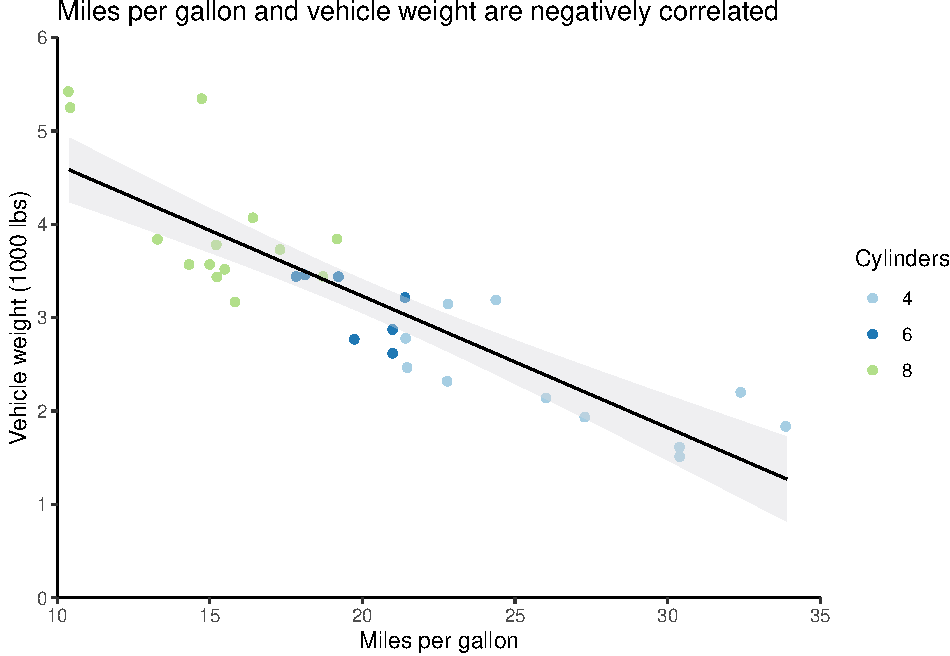
\includegraphics{rmarkdown-guide_files/figure-latex/content_graph_example-1.pdf}

A major aspect of \texttt{ggplot} that you should be aware of is that the plots are built in sequence. In the graph above (the code also appears below), \texttt{ggplot(mtcars)} came first, which just set up a blank graph, then there's \texttt{geom\_jitter}, which added the \texttt{wt} and \texttt{mpg} data and point colors based on the \texttt{cyl} variable, and so on. If I wanted the regression line from \texttt{geom\_smooth} to appear beneath the points rather than on top of them, I could've just reordered the function calls. This will also help you troubleshoot if you have issues outputting graphs; just comment out individual plot objects, being careful not to leave any dangling plus signs, and rerun to find the problem.

This functionality also means that you can save several layers in a list to apply them easily to multiple graphs. This can save you time and effort when you want to have a consistent look across different graphs; just update a particular parameter in your list once, and then it'll apply across your graphs.

Some functions, like \texttt{labs}, support this layering very well by allowing multiple calls to the same function. Others, like \texttt{scale\_y\_continuous}, will override previous calls in the same graph (you'll get a warning message when this happens). You'll notice that I have to put commas in between each function in the list rather than plus signs. I also have to save these in a \texttt{list}(rather than with \texttt{c}).

\begin{Shaded}
\begin{Highlighting}[]
\CommentTok{# Create list of specifications}
\NormalTok{format_list <-}\StringTok{ }\KeywordTok{list}\NormalTok{(}\KeywordTok{scale_y_continuous}\NormalTok{(}\DataTypeTok{expand =} \KeywordTok{c}\NormalTok{(}\DecValTok{0}\NormalTok{,}\DecValTok{0}\NormalTok{), }\DataTypeTok{limits =} \KeywordTok{c}\NormalTok{(}\DecValTok{0}\NormalTok{,}\DecValTok{6}\NormalTok{)),}
                    \KeywordTok{scale_x_continuous}\NormalTok{(}\DataTypeTok{expand =} \KeywordTok{c}\NormalTok{(}\DecValTok{0}\NormalTok{,}\DecValTok{0}\NormalTok{), }\DataTypeTok{limits =} \KeywordTok{c}\NormalTok{(}\DecValTok{10}\NormalTok{,}\DecValTok{35}\NormalTok{)),}
                    \KeywordTok{scale_color_brewer}\NormalTok{(}\DataTypeTok{type =} \StringTok{"qual"}\NormalTok{, }\DataTypeTok{palette =} \StringTok{"Paired"}\NormalTok{),}
                    \KeywordTok{theme_classic}\NormalTok{(),}
                    \KeywordTok{labs}\NormalTok{(}\DataTypeTok{y =} \StringTok{"Vehicle weight (1000 lbs)"}\NormalTok{,}
                         \DataTypeTok{x =} \StringTok{"Miles per gallon"}\NormalTok{,}
                         \DataTypeTok{color =} \StringTok{"Cylinders"}\NormalTok{))}

\CommentTok{# Create scatter plot}
  \CommentTok{# Move legend to the bottom}
\NormalTok{mtcars_scatter <-}\StringTok{ }\KeywordTok{ggplot}\NormalTok{(mtcars) }\OperatorTok{+}
\StringTok{  }\KeywordTok{geom_jitter}\NormalTok{(}\KeywordTok{aes}\NormalTok{(mpg, wt, }\DataTypeTok{color =}\NormalTok{ cyl)) }\OperatorTok{+}
\StringTok{  }\KeywordTok{geom_smooth}\NormalTok{(}\KeywordTok{aes}\NormalTok{(mpg, wt), }\DataTypeTok{method =} \StringTok{"lm"}\NormalTok{, }\DataTypeTok{se =} \OtherTok{TRUE}\NormalTok{, }\DataTypeTok{level =} \FloatTok{0.95}\NormalTok{, }
              \DataTypeTok{fill =} \StringTok{"#d7d8db"}\NormalTok{, }\DataTypeTok{color =} \StringTok{"black"}\NormalTok{, }\DataTypeTok{size =} \FloatTok{0.5}\NormalTok{) }\OperatorTok{+}
\StringTok{  }\NormalTok{format_list }\OperatorTok{+}
\StringTok{  }\KeywordTok{theme}\NormalTok{(}\DataTypeTok{legend.position =} \StringTok{"bottom"}\NormalTok{)}

\CommentTok{# Output scatter plot with new legend position}
\NormalTok{mtcars_scatter}
\end{Highlighting}
\end{Shaded}

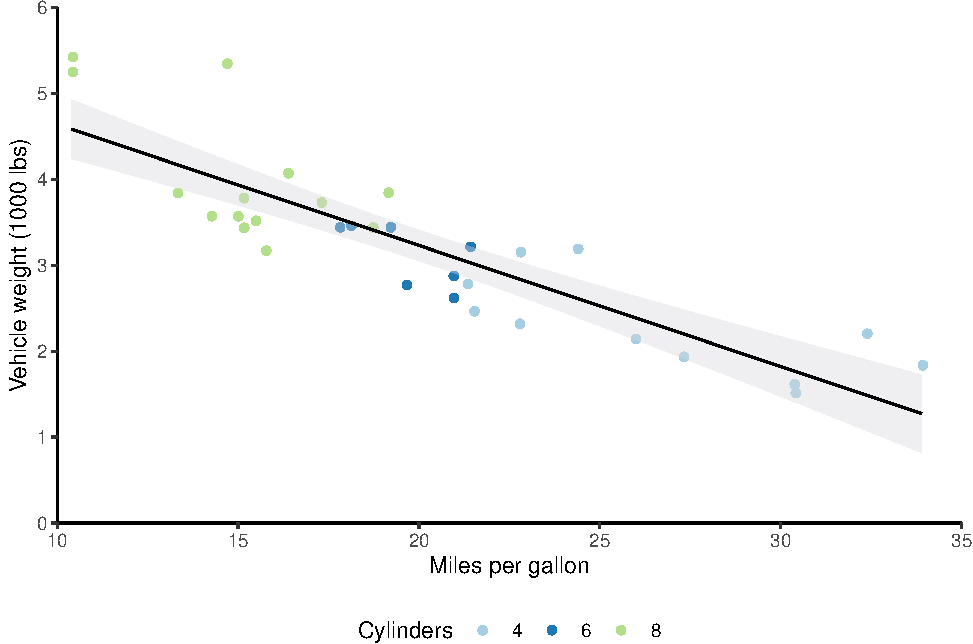
\includegraphics{rmarkdown-guide_files/figure-latex/content_graph_3-1.pdf}

You'll want to be familiar with the \href{https://colorbrewer2.org/}{color brewer palettes} that I used here. The website I've linked allows you to play with the different options and choose ones with particular characteristics, like color blind-friendly palettes. You can use the \texttt{scale\_color/fill\_brewer} functions with \texttt{ggplot} to apply these color palettes.

Relatedly, there's a difference between setting \texttt{fill} and \texttt{color} options in \texttt{ggplot}. Generally, scatter plots get \texttt{color} settings, while bar plots get \texttt{fill} settings. If I'd set \texttt{fill\ =\ cyl} in \texttt{geom\_jitter}, I would've gotten a legend with the three cylinder types, but the colors of the points wouldn't have changed. Similarly, if I'd used \texttt{scale\_fill\_brewer} rather than \texttt{scale\_color\_brewer}, the colors of the points would still have been the R defaults (or you would get an error, depending on the data type).

Lastly on formatting, you'll want to become familiar with the \texttt{theme} function as your graphs increase in complexity. The description for this function says it best: ``Themes are a powerful way to customize the non-data components of your plots: i.e.~titles, labels, fonts, background, gridlines, and legends.'' I typically layer \texttt{theme\_classic} with several \texttt{theme} specifications. Search \texttt{?theme} in your R console or Help window for the full list of parameters.

\hypertarget{visualizing}{%
\subsection{Visualizing}\label{visualizing}}

I often need to make bar graphs to present data. I also tend to want to include error bars on these bar graphs. There are different error bars you can calculate, but I tend to have error bars that represent 95\% confident intervals around my means. You'll first need to install the \texttt{Rmisc} package to do this, then transform your data into a long format. I also turned the categorical variables that I cared about into factors. This allows you to control the exact label text and order in your graph. Then, I used the \texttt{summarySE} function to create a table with the means and confidence intervals.

\begin{Shaded}
\begin{Highlighting}[]
\CommentTok{# Create long-form data for creating error table}
  \CommentTok{# Mutate columns to create factors with particular labels}
  \CommentTok{# This is harder to change once you're at ggplot stage}
\NormalTok{mtcars_long <-}\StringTok{ }\NormalTok{mtcars }\OperatorTok
\StringTok{  }\KeywordTok{select}\NormalTok{(mpg, wt, cyl) }\OperatorTok
\StringTok{  }\KeywordTok{pivot_longer}\NormalTok{(}\DataTypeTok{cols =} \OperatorTok{-}\NormalTok{cyl, }\DataTypeTok{names_to =} \StringTok{"variables"}\NormalTok{, }\DataTypeTok{values_to =} \StringTok{"measures"}\NormalTok{) }\OperatorTok
\StringTok{  }\KeywordTok{mutate}\NormalTok{(}\DataTypeTok{cyl =} \KeywordTok{factor}\NormalTok{(cyl, }\DataTypeTok{levels =} \KeywordTok{c}\NormalTok{(}\DecValTok{4}\NormalTok{, }\DecValTok{6}\NormalTok{, }\DecValTok{8}\NormalTok{), }
                      \DataTypeTok{labels =} \KeywordTok{c}\NormalTok{(}\StringTok{"4-cylinder"}\NormalTok{, }\StringTok{"6-cylinder"}\NormalTok{, }\StringTok{"8-cylinder"}\NormalTok{)),}
         \DataTypeTok{variables =} \KeywordTok{factor}\NormalTok{(variables, }\DataTypeTok{levels =} \KeywordTok{c}\NormalTok{(}\StringTok{"mpg"}\NormalTok{, }\StringTok{"wt"}\NormalTok{), }
                            \DataTypeTok{labels =} \KeywordTok{c}\NormalTok{(}\StringTok{"Miles per gallon"}\NormalTok{, }\StringTok{"Vehicle weight (1000 lbs)"}\NormalTok{)))}

\CommentTok{# Make error table}
\NormalTok{mtcars_error <-}\StringTok{ }\KeywordTok{summarySE}\NormalTok{(mtcars_long, }\DataTypeTok{measurevar =} \StringTok{"measures"}\NormalTok{, }\DataTypeTok{groupvars =} \KeywordTok{c}\NormalTok{(}\StringTok{"cyl"}\NormalTok{, }\StringTok{"variables"}\NormalTok{))}

\CommentTok{# Output error table}
\NormalTok{mtcars_error}
\end{Highlighting}
\end{Shaded}

\begin{verbatim}
##          cyl                 variables  N  measures        sd        se
## 1 4-cylinder          Miles per gallon 11 26.663636 4.5098277 1.3597642
## 2 4-cylinder Vehicle weight (1000 lbs) 11  2.285727 0.5695637 0.1717299
## 3 6-cylinder          Miles per gallon  7 19.742857 1.4535670 0.5493967
## 4 6-cylinder Vehicle weight (1000 lbs)  7  3.117143 0.3563455 0.1346860
## 5 8-cylinder          Miles per gallon 14 15.100000 2.5600481 0.6842016
## 6 8-cylinder Vehicle weight (1000 lbs) 14  3.999214 0.7594047 0.2029595
##          ci
## 1 3.0297434
## 2 0.3826381
## 3 1.3443253
## 4 0.3295647
## 5 1.4781278
## 6 0.4384672
\end{verbatim}

Now I can make a bar graph with this error table. My main \texttt{ggplot} object uses the \texttt{cyl} column and plots the means, while the \texttt{geom\_errorbar} object uses the confidence interval (\texttt{ci}) column to create the error bars. You'll also notice that I changed the width of the error bars and their position, so that they were centered over the bars.

\begin{Shaded}
\begin{Highlighting}[]
\CommentTok{# Create bar graph}
\NormalTok{mtcars_bar <-}\StringTok{ }\KeywordTok{ggplot}\NormalTok{(mtcars_error, }\KeywordTok{aes}\NormalTok{(cyl, measures, }\DataTypeTok{fill =}\NormalTok{ cyl)) }\OperatorTok{+}
\StringTok{  }\KeywordTok{geom_bar}\NormalTok{(}\DataTypeTok{position=}\StringTok{"dodge"}\NormalTok{, }\DataTypeTok{stat=}\StringTok{"identity"}\NormalTok{) }\OperatorTok{+}
\StringTok{  }\KeywordTok{geom_errorbar}\NormalTok{(}\KeywordTok{aes}\NormalTok{(}\DataTypeTok{ymin =}\NormalTok{ measures }\OperatorTok{-}\StringTok{ }\NormalTok{ci, }\DataTypeTok{ymax =}\NormalTok{ measures }\OperatorTok{+}\StringTok{ }\NormalTok{ci), }
                \DataTypeTok{width =} \FloatTok{0.1}\NormalTok{, }\DataTypeTok{position =} \KeywordTok{position_dodge}\NormalTok{(}\FloatTok{0.9}\NormalTok{)) }\OperatorTok{+}
\StringTok{  }\KeywordTok{coord_flip}\NormalTok{() }\OperatorTok{+}
\StringTok{  }\KeywordTok{scale_y_continuous}\NormalTok{(}\DataTypeTok{expand =} \KeywordTok{expand_scale}\NormalTok{(}\DataTypeTok{mult =} \KeywordTok{c}\NormalTok{(}\DecValTok{0}\NormalTok{, }\FloatTok{.2}\NormalTok{))) }\OperatorTok{+}
\StringTok{  }\KeywordTok{scale_fill_brewer}\NormalTok{(}\DataTypeTok{type =} \StringTok{"qual"}\NormalTok{, }\DataTypeTok{palette =} \StringTok{"Paired"}\NormalTok{) }\OperatorTok{+}
\StringTok{  }\KeywordTok{theme_classic}\NormalTok{() }\OperatorTok{+}
\StringTok{  }\KeywordTok{facet_wrap}\NormalTok{(}\OperatorTok{~}\StringTok{ }\NormalTok{variables, }\DataTypeTok{scales =} \StringTok{"free_x"}\NormalTok{) }\OperatorTok{+}
\StringTok{  }\KeywordTok{labs}\NormalTok{(}\DataTypeTok{y =} \StringTok{"Measures"}\NormalTok{,}
       \DataTypeTok{x =} \StringTok{"Cylinders"}\NormalTok{,}
       \DataTypeTok{fill =} \StringTok{"Cylinders"}\NormalTok{) }\OperatorTok{+}
\StringTok{  }\KeywordTok{theme}\NormalTok{(}\DataTypeTok{axis.ticks.y =} \KeywordTok{element_blank}\NormalTok{(),}
        \DataTypeTok{legend.position =} \StringTok{"none"}\NormalTok{,}
        \DataTypeTok{panel.spacing.x =} \KeywordTok{unit}\NormalTok{(}\FloatTok{1.5}\NormalTok{, }\StringTok{"lines"}\NormalTok{),}
        \DataTypeTok{axis.text.y =} \KeywordTok{element_text}\NormalTok{(}\DataTypeTok{angle =} \DecValTok{90}\NormalTok{, }\DataTypeTok{hjust =} \FloatTok{0.5}\NormalTok{))}

\CommentTok{# Output bar graph}
\NormalTok{mtcars_bar}
\end{Highlighting}
\end{Shaded}

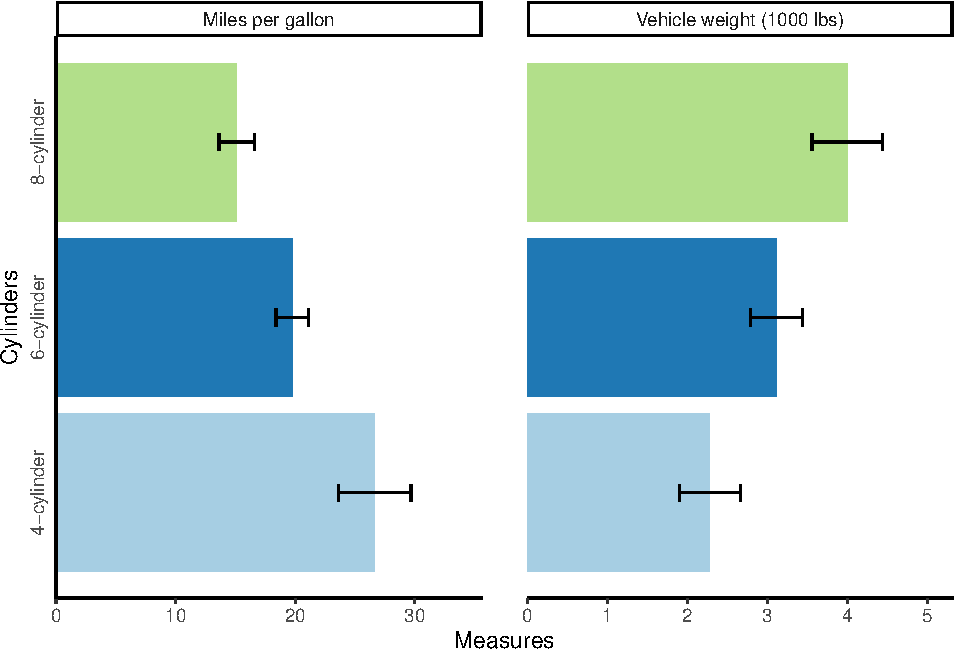
\includegraphics{rmarkdown-guide_files/figure-latex/content_graph_5-1.pdf}

Sometimes, you'll want to output multiple graphs with a particular layout. The \texttt{patchwork} package allows you to do this easily. The syntax is very similar to \texttt{ggplot} syntax, in that you add plots together with a plus sign. You can also add a \texttt{plot\_layout} object to change aspects of the plots, like their widths.

\begin{Shaded}
\begin{Highlighting}[]
\NormalTok{ mtcars_bar }\OperatorTok{+}\StringTok{ }\NormalTok{mtcars_scatter }\OperatorTok{+}\StringTok{ }\KeywordTok{plot_layout}\NormalTok{(}\DataTypeTok{widths =} \KeywordTok{c}\NormalTok{(}\DecValTok{2}\NormalTok{, }\DecValTok{1}\NormalTok{))}
\end{Highlighting}
\end{Shaded}

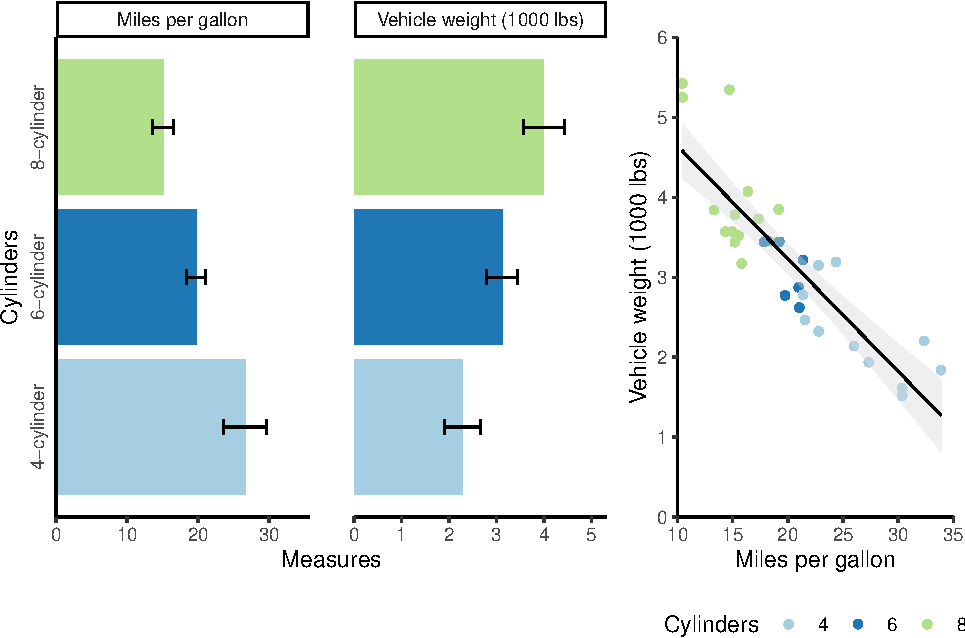
\includegraphics{rmarkdown-guide_files/figure-latex/content_graph_6-1.pdf}

\hypertarget{practice-materials}{%
\section{Practice materials}\label{practice-materials}}

You can find practice materials for R Markdown and R \href{https://github.com/hollzzar/markdown-tutorial}{here}. You'll want to clone this repository or download the following documents/folders:

\begin{itemize}
\tightlist
\item
  brownbag\_activity.Rmd
\item
  data\_cleaning.R
\item
  apa.csl
\item
  /data
\end{itemize}

  \bibliography{packages.bib}

\end{document}
